%!TEX root = ../PhDthesis.tex
\chapter{Literature Review}


\section{Early Visual System}

The early stages of mammalian visual system (pictured in figure
\ref{VisualSystem}) consist of the retina, where rod and cone
photoreceptors convert incident photons into electrical and chemical
signals. These signals are then further converted from analogue
voltages into spike trains by retinal bipolar and ganglion cells and
sent down the optic nerve to the lateral geniculate nucleus
(LGN). Connections from the two eyes cross over at the optic chiasm to
form projections of the right and left visual field
contra-laterally. The connections from the retina map retinotopically
onto the LGN, which ensures that nearby areas of LGN respond to nearby
portions of the visual field. After the initial processing in the
retina and LGN the visual stream is projected onto the primary visual
cortex (V1).

\begin{figure}
	\centering
        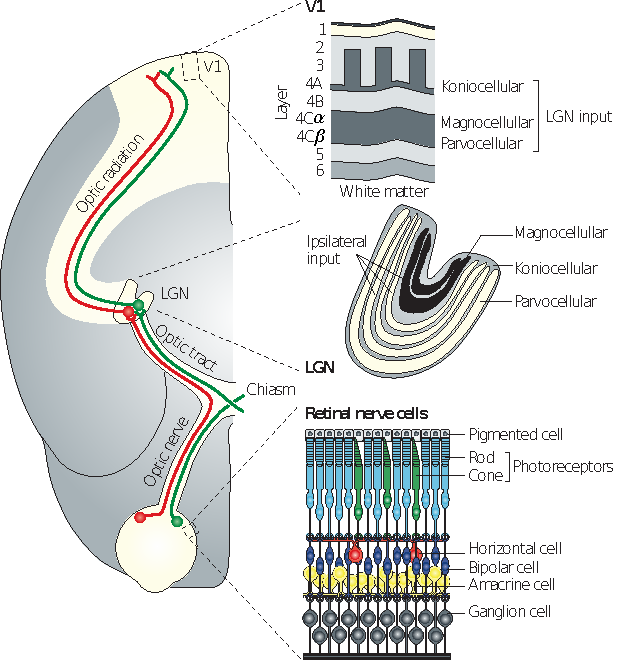
\includegraphics[width=0.9\textwidth]{solomon.pdf}
	\caption{The early visual pathway in primates (at least
          superficially the same for most other mammals) from the
          retina to the primary visual cortex (V1) via the lateral
          geniculate nucleus (LGN) of the thalamus. The left panel
          shows the pathway, while the right panels highlight
          noteworthy sections including the structure of the retina,
          the LGN and V1 broken down into their different layers and
          showing different cell types. Reprinted from
          \cite{Solomon2007}.}
	\label{VisualSystem}
\end{figure}

Retinal processing begins, as previously mentioned, with the
photoreceptors, which release glutamate into the synaptic terminal
connecting them to bipolar or horizontal cells. The bipolar cells
respond either as ON or OFF cells as the glutamate either de- or
hyperpolarizes them basically turning on or off in response to light
stimulation. The bipolar cells can make connections to a small or
large number of photoreceptors or even be indirectly connected to them
via horizontal cells, which leads to a large variance in receptive
field size and structure.

In the retina, summation of various photoreceptor types gives rise to
so called center-surround receptive fields. These ON- and OFF-center
receptive fields can arise in bipolar cells but are more commonly
associated with retinal ganglion cells (RGCs). This receptive field
type responds most strongly to spots of light/dark moving through the
visual field (as shown in figure \ref{Center-Surround}) but can be
characterized as simple edge detectors.

\begin{figure}
	\centering 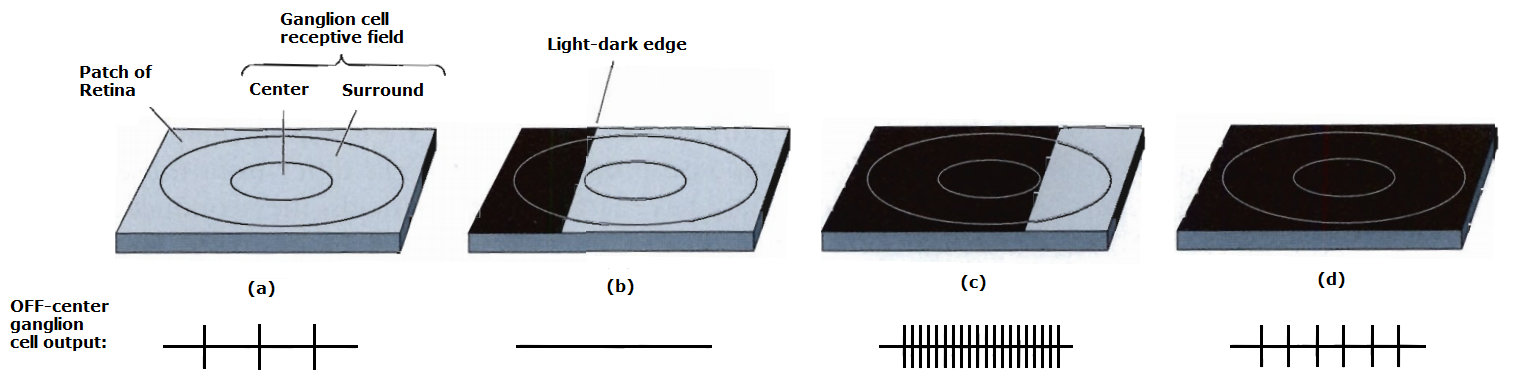
\includegraphics[width=0.9\textwidth]{Figure2.png}
	\caption{The centre-surround receptive field
        structure of some retinal ganglion cells and LGN neurons,
        illustrating how a contrast edge activates different portions
        of the field and thereby results in different activation
        patterns. From left to right one can see that as the
        light-dark edge moves into the ON surround field spontaneous
        activity is suppressed and as it moves further over the OFF
        center field is deactivated causing activity to sharply
        spike. Adapted from \cite{Bear2006}.}
	\label{Center-Surround}
\end{figure}

Much like the retina and many other areas of the brain, the LGN forms
a laminar architecture, receiving input from RGCs and projecting axons
to the primary visual cortex via the optic radiation. The separation
of LGN cells into layers also corresponds to functional separations,
as layers 1, 4 and 6 usually receive contra-lateral input, while
layers 2, 3 and 5 receive ipsi-lateral inputs from the
retina. Furthermore, different layers consist of different cell types,
with ventral layers 1 and 2 containing larger so called magno-cellular
(M) neurons and dorsal layers 3, 4, 5 and 6 containing smaller
parvo-cellular (P) neurons with intra-laminar neurons being referred
to as konio-cellular (K). Since these three cell types are also
present in the retina and make connections mainly with their own cell
type it is theorized that each carries its own parallel information
stream. Functionally, P-cells have displayed greater sensitivity to
chromatic contrast and higher spatial frequencies, linking them to the
processing of detail and color, while M-cells have been shown to have
greater sensitivity for high temporal frequencies associating them
with motion processing.  In addition to the feedforward retinal input,
the LGN also receives feedback connections from V1, the influence of
which has not yet been fully clarified but will be explored later on.

\subsection{Primary Visual Cortex: Topographic Maps, Simple and Complex Cells}

The primary visual cortex (V1) or striate cortex provides the first
cortical stage of processing of visual information. The cortex was
classically divided into six layers but since many subdivisions have
been added after functional sub-groups were discovered. Feedforward
input from the LGN is received in layer 4C$\alpha$ and 4C$\beta$ ,
which receive input most of their input from M- and P-cells
respectively. The neurons in layer 4 then send projections up to
layers 2/3, which has a diverse intralaminar network of connections
but also sends intracortical projections to a number of higher visual
areas, while layers 5 and 6 provide feedback to the LGN.

Neurons in the primary visual cortex (V1) are tuned to respond to a
variety of different features or complex combinations of such
features, including orientation, spatial and temporal frequency,
motion direction, colour or ocular origin. In many mammal species
especially primates and carnivores, these feature preferences map
smoothly and topographically onto the cortical surface. This mapping
extends vertically through the layers of the cortex, giving rise to
the notion of distinct cortical columns. Retinotopy arises due to the
mapping of visual information straight from the retina to the LGN and
then to the cortex. Other response preferences such as orientation and
direction selectivity rarely arise in the LGN and are usually thought
of as an emergent phenomenon in the cortex.

\begin{figure}
	\centering 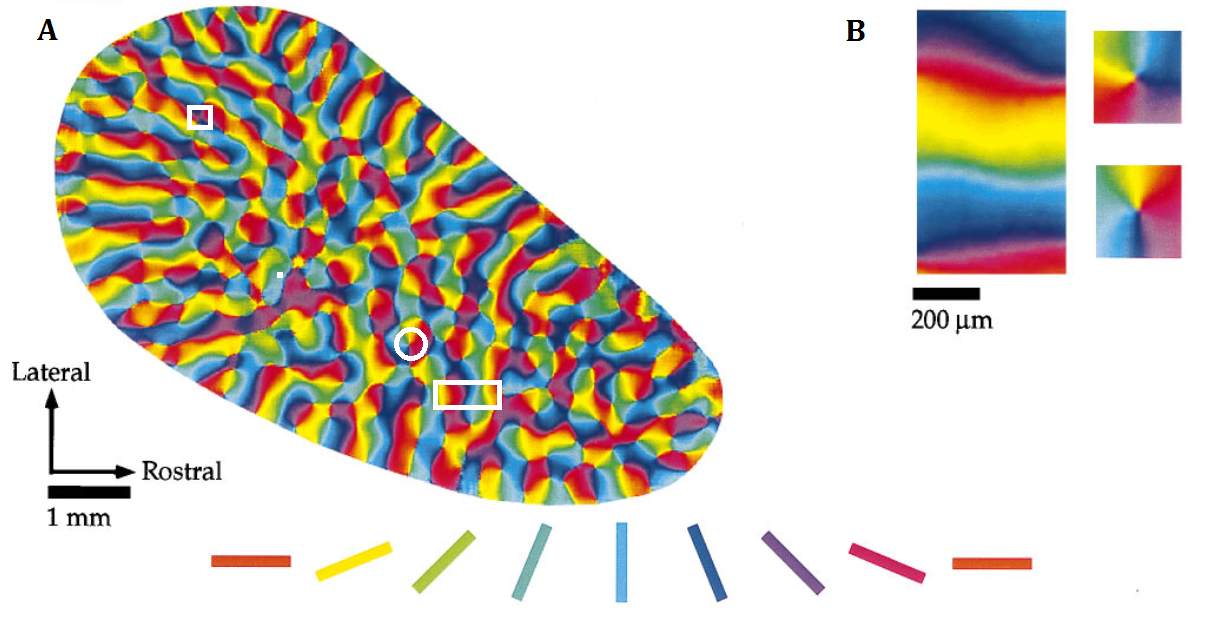
\includegraphics[width=0.9\textwidth]{Figure3.png}
	\caption{A) Orientation preference map in a ferret generated
          by overlaying the activity maps for different orientations
          and artificially colouring each area according to the
          orientation preference laid out in the legend below. The
          image also highlights three recurrent features of
          orientation maps in white. The square highlights a saddle
          point, where a patch of cortex selective for a particular
          direction is almost bisected by a patch selective to another
          direction. The circle highlights a pinwheel arrangement,
          where different orientations preference patches are arranged
          in a circular shape. Finally the rectangular shape
          highlights a linear zone in which orientation preference
          change continuously. B) Magnifications of a linear zone and
          two pinwheel arrangements. Adapted from \cite{Bosking1997}.}
	\label{OrientationMap}
\end{figure}

The receptive fields of V1 neurons are different in that often are no
longer simple ON- or OFF-centre surround fields, forming more complex
spatiotemporal patterns. They are commonly modeled using Gabor filters
as shown in Figure \ref{Gabor}, which have elongated ON and OFF
regions or lobes, generated by localizing a full-field sine grating
with a Gaussian envelope. Orientation selectivity and spatial
frequency preference are determined by the orientation and spacing of
ON- and OFF-regions respectively. It is also possible for V1 cells to
filter temporal patterns by employing spatio-temporal shifts in their
ON and OFF lobes, giving rise to direction selectivity.

Orientation selective neurons can generally be classed as simple or
complex cells, depending on whether they display some form of
spatial/phase invariance. In reality this classification is less clear
with cells being somewhere on a gradient from pure simple cells to a
complex cell with the degree of phase invariance being the determining
factor. Apart from phase invariance the neurons may also exhibit
contrast invariance, such that even at very low contrast they will
respond more strongly to their preferred orientation than to the
orthogonal orientation.

\begin{figure}
	\centering 
\includegraphics[width=0.25\textwidth]{gabor.png}
        
\includegraphics[width=0.25\textwidth]{gabor90.png}
	\caption{Gabor Patches at 0 degree and 90/180 degree
          orientations with clearly visible ON (white) and OFF (black)
          regions.}
	\label{Gabor}
\end{figure}

In context of this project topographic feature maps and RF
interactions play a fundamental role as they provide the basis around
which the neural circuit organize. The functional organization of V1
arises during the development of the animal and are thought to be
mediated largely by activity dependent processes as the next section
will show.

\subsection{Development of Topographic Maps in V1}

The development and maturation of cortical topographic feature
representations in the form of maps is closely linked to function and
can reveal a lot about how the cortex is capable of capturing and
encoding statistics of the natural world. Developmental studies
involve imaging the same area of the cortex over a number of days and
investigating what drives development of orientation maps and other
topographic arrangements. Early developmental studies found, using
relatively limited optical imaging techniques on ferrets shortly after
eye opening, that the iso-orientation domains in the V1 develop very
early in development and subsequently show very little change
\citep{Chapman1996} (pictured in figure \ref{RFMapDevelopment}). These
and other experiments \citep{White2007} showed that orientation
preference develops even in absence of visual input although the maps
do not fully mature. This seems to suggest that orientation maps and
other topographic organizations develop initially even in absence of
external visual input through internally generated visual activity
such as retinal waves but then require external stimulation to fully
mature.

\begin{figure}
	\centering 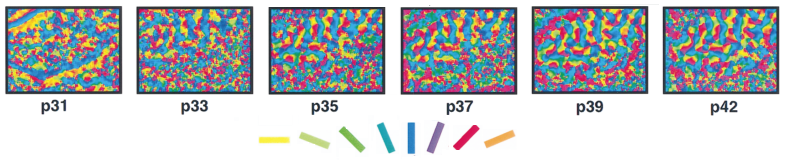
\includegraphics[width=0.9\textwidth]{Figure6.png}
	\caption{Development of orientation map in ferret visual
          cortex from postnatal day 31 to 42 revealed using chronic
          optical imaging of intrinsic signals. Adapted from
          \citep{Chapman1996}.}
	\label{RFMapDevelopment}
\end{figure}

In the initial stages of development various preprogrammed guidance
cues set up the basic connectivity between the LGN and the cortical
processing areas. Some successful models of development have focused
on the afferent connections between the LGN ON and OFF cells and their
targets in the visual cortex as the driving force behind the
development of orientation columns \citep{Jin2011}. This is likely to
tell only part of the story as even during prenatal development,
retinal waves, consisting of periodic activity in retinal ganglion
cells (RGCs), spread across the retina driving neighboring RGCs to
fire in a correlated fashion, which allows the primary visual cortex
to develop topographic feature maps \citep{Firth2005}. The most
prominent proposals in theory and in models have been focused the
termination pattern of both the geniculocortical afferents in layer 4
\citep{Katz2000,Ringach2007} and adjustments in feedforward and
lateral connectivity through activity dependent, competitive processes
\citep{Bednar2003}.

It is now generally accepted that the development of topographic maps
is driven activity dependent weight modification in form of Hebbian
learning or some variant thereof \citep{Wolf}. The LISSOM and
GCAL models, which provide the basis of the modeling work proposed in
this project have shown that robust map development can be achieved
with a small number of relatively simple mechanisms including
homeostatic plasticity, lateral gain control in LGN and lateral
connectivity in V1 \citep{Stevens2013} and will be considered in more
detail at a later stage. These models can account for the development
of orientation preference maps through both intrinsic activity such as
retinal waves \citep{Bednar2003} and visually induced retinal
activity. Experiments show that at the very least these processes are
required to achieve the finely tuned precision, which can now be
observed at single cell resolution \citep{Ohki2005,White2007}.

Lateral intra-areal connections in particular have been implicated in
map development as their functional connectivity seems to be closely
related to map structure \citep{Gilbert1983}. Experiments in layer 2/3
of the tree shrew involving orientation preference mapping and
subsequent axonal staining have shown that although short range
connections show no preference in their terminations, long range
connections longer than 500 \si{\micro\metre}, preferentially link
neurons with co-oriented and co-axially aligned receptive fields
\citep{Bosking1997}. In iso-orientation regions cells therefore make
short-range connections largely with cells that prefer the same
direction as them, while the connectivity at pinwheels short-range
connections are made with cells with a wide range of orientation
preferences \citep{Ohki2006a}. However, it is known that the patchy
lateral connectivity in V1 does not arise until after the orientation
map has emerged \citep{Ruthazer1996}, indicating that they may be
involved in some higher-order processing not required during initial
development.

The development of the early visual pathway is probably driven by a
number of mechanisms complementing each other at various stages
starting with guidance cues setting up coarse predetermined
connectivity patterns, which are then refined through Hebbian
processes driven by in- and extrinsically stimulated
activity. Although the structure of a neurons receptive field is
constantly changing and varies widely from cell to cell, a lot of work
has gone into measuring the exact structure and functional properties
of neural receptive fields and their underlying anatomical correlates,
the neurite arbors.



\section{Developmental models of the Primary Visual Cortex}

As it is thought that the cortex captures statistics about the sensory
streams to construct internal models of the world, it is clear that
function, structure and development are closely linked. Recognizing
this close association, Dr. Bednar began developing models of the
sensory cortex \citep{Bednar2003} based on self-organizing maps
(SOMs). Since then these models have been refined substantially but
still implement the retina, LGN and V1 as a set of neuronal sheets
with feedforward and lateral connectivity self-organizing into the
complex topographic maps as seen in carnivore and primate species. It
can explain the development of robust yet adaptive topographic maps
using only a small set of mechanism including contrast-gain control,
an adaptive single-neuron threshold, and lateral connectivity giving
rise to GCAL \citep{Law2011}. Extensions of this model explaining the
development of complex cells and of contrast dependent size tuning
\citep{Antolik2011} as well as a continuous time model incorporating
LGN/V1 onsets using hysteresis functions are in development
\citep{Stevens2011}.

The GCAL model is based on several core observations about
information-processing in V1 and the cortex in general. As previous
sections have shown, the primary visual cortex of primates responds
strongly to specific low-level features in its visual input including
orientation, color and direction. Selectivity to these features are
conserved across a wide range of contrasts and neurons form
topographic feature maps across the surface of V1 by virtue of
self-organization. While these experimentally confirmed findings are
specific to vision, the concept of equipotentiality proposes that
different areas in the cerebral cortex are cytoarchitectonically
highly similar, becoming differentiated based largely on the
statistical patterns in their inputs during development and are thus
capable of capturing any sensory modality. While details surrounding
this hypothesis are still controversial, experiments such as those by
\cite{Sur1990} have at least partly validated this view. In this
particular study, experimentalists rewired optic nerve axons to
interface with neurons in the medial geniculate nucleus (MGN), part of
the pre-cortical auditory pathway, and subsequently showed that
neurons in the primary auditory cortex (A1) would become receptive to
features usually associated with V1. This is behind much of what has
made V1 such a popular model area for neuroscience and suggests that
many of the insights that can be gleaned from the study of V1 could be
applied to the cortex as a whole.

\begin{figure}
	\centering 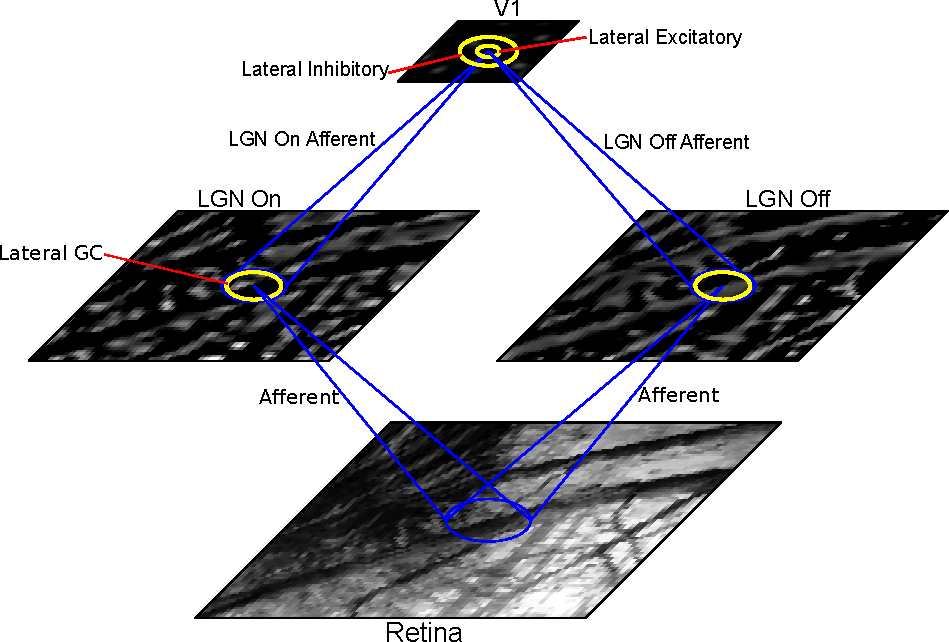
\includegraphics[width=1.0\textwidth]{GCAL.pdf}
	\caption{Schematic of simplest GCAL model for development
        of simple cells with surround modulation, retinotopic
        organization and orientation preference maps. It consists of a
        retinal sheet, two RGC/LGN for ON and OFF cell responses and
        one V1 sheet, connected with intra- and inter-areal
        projections. The sheets are drawn to scale, with larger sheets
        for the RGC/LGN and retinal layers to avoid edge
        effects. Projections are illustrated with blue (feedforward
        connections) and yellow (lateral connections) ovals with cones
        converging on their target, all drawn to scale to show their
        spatial extents. RGC/LGN sheets consist of units with
        hardwired Difference of Gaussian RFs with ON and OFF
        center-surround regions. LGN Afferent projections to V1 are
        initially unspecific but develop Gabor-like RF structures
        through Hebbian learning as they are observed experimentally.}
	\label{GCAL}
\end{figure}

The architecture of the GCAL model in its simplest form and as it will
initially be used in this project relies on only four sheets, a
retinal sheet for the presentation of stimuli, two RGC/LGN sheets and
a V1 sheet. These sheets are connected with different intra- and
inter-areal connection fields. This simple model can only be used to
demonstrate retinotopy, orientation preference and the emergence of
simple cell-like RFs but more complex models have been shown to
additionally account for complex cells, ocular dominance, motion
direction, spatial frequency, temporal frequency, disparity and
color. All these models are trained by presenting it with a visual
input on the retina, allowing the response to propagate through the
different sheets and then adjusting the connections weights to V1
neurons based on a local learning rule. The response of a given neuron
$j$ at time $t+\delta t$ can be calculated as the thresholded dot
product between the activations of every input neurons $i$ at time
$t$, or $\eta_i(t)$, and their associated weights stored in the
connection field:

\begin{equation}
\eta_j(t+\delta t) = \sigma \left ( \sum_p{\gamma_p} \sum_{i \in
  F_{jp}}{\eta_i(t)\omega_{ij}}\right)
\end{equation}

where $\eta_i$ is the activation of all units $i$ in connection field
$F_{jp}$, which contains all neurons unit $j$ receives its inputs
from. $\omega_{ij}$ is the connection weight from $i$ to $j$. $\sigma$
is a half-wave rectifying function with a variable threshold point
($\theta$) dependent on the average activity of the unit, effectively
acting as a homeostatic mechanism, pulling the activity of neuron back
to a desired level. $\gamma_p$ is an arbitrary multiplier for the
overall strength of all connections $i$ in projection $p$ and thus a
free parameter.

The connection weights $\omega_{ij}$ are adjusted after each iteration
using a simple Hebbian learning rule, capturing correlations between
pre- and post-synaptic activities. The Hebbian connection weight
update for unit $j$ is expressed as a function of the presynaptic
activity $\eta_i$, the post-synaptic response $\eta_j$ and the Hebbian
learning rate $\alpha$, taking the form:

\begin{equation}
\omega_{ij}(t+1) = \frac{\omega_{ij}(t) + \alpha \eta_j
  \eta_i}{\sum_{k\in F_jp}{ (\omega_{kj}(t) + \alpha \eta_j \eta_k)}}
\end{equation}

This function also constrains runaway changes in weights by employing
divisive post-synaptic weight normalization and thus eliminates the
instability associated with classical Hebbian learning.

This limited number of mechanisms already gives rise to an incredibly
robust model of development of topographic map development and
generates different experimentally observed RF profiles. To add
further robustness to the model and to allow it to respond across a
wide range of contrasts, contrast-gain control was introduced in the
LGN sheets (marked as Lateral GC). This mechanism was closely modeled
on the divisive normalization model introduced and validated by
\cite{Bonin2005}. Finally, the lateral excitatory and inhibitory
fields in the V1 sheet give rise not only to the topographic map
structure but also to some surround modulation effects. In particular,
it can explain the size tuning properties of V1 neurons as the
excitatory field will boost the response to a growing centered disk up
to a certain peak, after which point the lateral inhibitory field
dominates and reduces the response to the stimulus as it grows
further. It may also explain effects such as iso-orientation
suppression but this has as of yet not been explored in detail.

Overall, due to the simplicity of its mechanisms and its explanatory
strength, GCAL provides an ideal starting point to explore the
contribution of feedforward, lateral and feedback components to V1,
how bottom-up attention can arise and how top-down attention can
modulate the processing architecture.

\subsection{Functional and Anatomical Properties of Neural Receptive Fields}

The spatial properties of RFs in the LGN and V1 are of particular
interest in the context of this PhD project as they provide the basis
of a realistic model of the para-foveal regions of the primary visual
cortex in macaques, allowing direct comparisons between model in
experiment in a system where the spatial scales are of great
importance. Before attempting to model the effects of higher- and
extra-cortical influences on information processing in V1, the spatial
properties of each set of afferent connections entering V1 need to be
thoroughly understood and incorporated into the model.

The extents and structure of neural receptive fields are defined by
the axonal and dendritic arborization of afferent, horizontal and
feedback connections, whether that is in the LGN, the V1 or higher up
in the cortical architecture. While these extents can theoretically be
measured physically by tracing the neurites of a number of cells, this
has only systematically been possible for corticogeniculocortical
neurite complex as tracing studies along the retinal-geniculate
pathway are generally infeasible. Therefore spatial properties of LGN
RFs have been estimated through stimulus driven protocols. The
following sections will outline the methods employed in characterizing
geniculate RFs and detail the relative contribution of afferent,
lateral and feedback connections to para-foveal RFs in the LGN and V1
of macaques.

\subsubsection{Receptive Fields in the Lateral Geniculate Nucleus}
\label{sec:LGNRF}

The spatiotemporeal structure of receptive field becomes increasingly
more complex when moving up in the visual processing hierarchy. As
described earlier, receptive fields in the LGN are primarily made up
of antagonistic center-surround regions although Gabor-like lobes are
also sometimes observed. Even at this early stage of processing,
lateral and feedback connections can modulate neural responses and
have been found to exert a suppressive effect \citep{Hubel1961}. More
recent studies have concluded that this suppressive effect is mediated
primarily by lateral connections and acts as a form of contrast-gain
control allowing for the encoding of a high dynamic range of luminance
values \cite{Bonin2005}. As pointed out previously the LGN receives a
large proportion of its inputs from feedback cells originating in
layer 6 of V1 \citep{Sherman2002}. It is unclear how these feedback
connections contribute to the RF properties of LGN neurons but most
evidence suggests they are mainly involved in higher level modulatory
processes especially in regard to the processing of motion and thus do
not directly contribute to the RF structure \citep{Sillito2006}.

Estimating the relative contribution and effect of the various LGN
afferents on its neural receptive fields has been attempted using a
variety of protocols. Unfortunately little to no data is available
from tracing studies, primarily because the LGN is embedded deep in
the brain making it incredibly difficult to trace individual neurites
from and to their origin. Therefore a number of protocols were
developed by which the parameters of the center-surround fields could
be estimated. After measuring the response of retinal ganglion cells
(RGCs) to moving bar stimuli cats \citep{Rodieck1965a,Rodieck1965b},
\cite{Rodieck1965} found that by fitting a Difference of Gaussian
(DoG) model (see \ref{DoGf}) to the data it was possible to estimate
the relative strength and size of the central and surround portions of
the receptive field. It wasn't until later that systematic recordings
of this kind were carried out in the LGN of macaques at which point
the moving bar stimuli were replaced with sine gratings of varying
spatial frequency.

\begin{equation}
R = k_c e^{-\frac{f}{f_c}^2} - k_s e^{-\frac{f}{f_s}^2}
\label{DoGf}
\end{equation}

As not all papers can be considered, the data from three different
studies making use of protocols with increasing complexity will be
considered. \cite{Derrington1984} was the first of such studies,
attempting to characterize the spatial and temporal properties of
parvocellular LGN neurons in \emph{Macaca mulatta} by fitting DoG
models to the responses. The analysis and confidence intervals of this
first study were rather limited so the first study that will be
considered here is \cite{Spear1994}, which also considered the effect
of aging on receptive field properties. They found that the receptive
field center radius only increased very weakly with eccentricity, the
smallest RF center radii were confined to parvocellular neurons and
that the RF surround was significantly smaller in parvocellular
layers. This provides a first estimate for the mean sizes of the
central and surround portions of the classical RFs in macaque but the
clear problem with this approach is that it completely ignores the
influence of the non-classical surround and therefore may
underestimate the extents of the central field, while overestimating
the strength of the classical RF surround.

The next detailed study of LGN neural RFs was carried out by Levitt et
al. \cite{Levitt2001}, investigating the effects of visual deprivation
on their visual response properties. The study additionally set out to
determine the trans-species correspondence of so called X, Y and W
pathways, which were identified in the cat. As in the \cite{Spear1994}
study they found little difference in RF center radii between parvo-
and magnocellular neurons. They also found that magnocellular neurons
had greater nonlinearity indices but could find no compelling evidence
that magnocellular neurons can be classified into distinct linear (X)
and nonlinear (Y) types. There was a tendency for parvocellular
neurons to exhibit greater spatial resolution and the highest temporal
resolution to be magnocellular. This seems to support the general
conclusion reached by \cite{Derrington1984}, which had additionally
concluded that magno- and parvocellular neurons can be further
identified by their chromatic properties.  Finally, their analysis
extended to earlier data from different species of macaque, which
showed that there is some variation in the distribution of ON and OFF
cells between \emph{M. mulatta} and \emph{M. fascularis}. Overall
their results on spatial tuning match those found by previous studies
quite closely, which is unsurprising as the measuring and fitting
protocols were highly similar.

In an attempt to calculate the relative contributions of different
neural connections, determine differences between the K-, M- and
P-cellullar pathways and measure contrast dependent tuning, a number
of more recent studies have introduced more complex measurement and
fitting protocols. In particular, these experiments for the first time
attempted to separate out the influence of the non-classical or
extra-classical surround (ECRF or nCRF), which is thought to be
mediated by lateral and feedback connections. Therefore, a new
measurement and fitting protocol, introduced by \cite{Sceniak1999} in
form of the integrated DoG (iDoG) model to describe spatial summation
in the visual cortex, was used. Instead of measuring the response to
varying spatial frequency, this protocol involves the presentation of
drifting sine grating disks with varying apertures at the neurons
optimum spatial frequency. The rationale behind this new protocol was
that the optimal spatial frequency would maximally drive the CRF
excitatory center, while minimizing the influence of the CRF
surround. Therefore the resulting area summation tuning curve would
represent only the response from the CRF excitatory center and the
ECRF surround. Additionally the spatial frequency response measurement
protocol was modified by confining the drifting sine gratings to a
circular aperture, reducing influences from beyond the CRF. While
these assumptions do not necessarily hold for reasons that will be
discussed later, they provide a first systematic attempt at separating
the contributions from the CRF and ECRF.

\cite{Sceniak2006} were the first to study spatial RF properties of
LGN neurons of macaques by measuring both spatial frequency and area
summation response functions and fitting the results with DoG and iDoG
models respectively to estimate the spatial parameters of the probed
neurons. These results represent the best estimates of the spatial
properties of LGN receptive fields. The first thing to note is the
clear discrepancy between the estimates of CRF excitatory center
radius estimates in this paper compared to previous estimates. This
may be explained by the more homogenous distribution of cells as the
sample population was taken exclusively from layer 4. Additionally the
older protocol failed to confine the drifting sine grating to a disk,
which may have resulted systematic underestimation of the excitatory
component due to suppressive effects. While excitatory extents vary
hugely across the various studies the suppressive surround estimates
are fairly consistent. Furthermore, the spatial extent of the
excitatory CRF centers were found to be contrast invariant, while both
the ECRF and CRF suppressive surround extents were found to increase
at lower contrast levels. In summary, looking back at all the studies
considered here excitatory CRF extents are generally distributed
between 0.05-0.5$\degree$ in radius, while inhibitory CRF and
suppressive ECRF radii are distributed distributed anywhere between
0.6-1.5$\degree$ and the suppression index is quite high
(SI\textgreater0.8) for 80\% cells.

While these results provide the best estimates that are currently
available the protocols used rely on a number of flawed
assumptions. The DoG model fitted to the spatial frequency tuning
curve relies on the assumption that no other components are
contributing to the response. Although the limited size of the sine
grating disk drive should reduce long range influences on the response
and the ECRF surround is frequency invariant over a broader spectrum
than the CRF, further contributing mechanisms cannot be excluded and
may therefore affect the estimates. Similarly the iDoG model fitted to
area summation tuning curves may be affected by a number of
unaccounted mechanisms. Additionally the iDoG model (see \ref{iDoG})
actually corresponds to an even luminance disk of variable size rather
than the sine grating disks that were used by \cite{Sceniak2006}. The
decision to use technically incorrect stimuli was made to minimize the
influence of the inhibitory CRF surround, which may itself still have
some influence on the response. While all these limitations should be
held in mind, it is still the best attempt at controlling unaccounted
contributions and thus provides the best data on the spatial
properties of macaque LGN RFs until detailed histological studies
become feasible.

\subsubsection{Receptive Fields in the Primary Visual Cortex}

The receptive field properties of neurons in V1, in contrast to LGN
neurons, have been characterized to a far greater extent with a number
of studies publishing direct anatomical data on neurite arborization
in addition to studies involving stimulus protocols such as those
employed to characterize LGN RFs. A number of reviews have been
published in the past decade to classify different portions of the
receptive field and link them to their physiological substrate in the
form of feedforward (FF), lateral and feedback (FB) connections. In
order to attain a proper understanding of the spatial distribution of
afferent neurites, populations of V1 neurons are targeted by, this
section will summarize the results.

Recent analyses have established a more complex model for the
classification of the spatial properties of neural RFs in V1 than the
simpler classical and extra-classical RF structure utilized in earlier
work. The structure of a V1 receptive field has been visualized by
\cite{Angelucci2006a} and can be seen in Figure \ref{RFstruct}. It is
broken down into the minimum response field (mRF), the summation
response field (sRF), which itself is broken down into the high
contrast and low contrast summation RF (hsRF and lsRF) and the far
surround. In particular, a distinction has been made between the near
surround, which extends as far as the lsRF and a suppressive far
surround that extends beyond the lsRF. The distinction between the
hsRF and lsRF has been introduced to account for the contrast
dependence of size tuning. Problematically not all studies nor even
all the latest studies use this means of defining different portions
of the RF, which may have led to discrepancies of how the sizes of
different RF areas are reported. The following sections will attempt
to integrate the results from studies employing different means of
classifying RFs.

The studies reviewed in \cite{Angelucci2006a} seem to indicate that
geniculocortical FF projections integrate signals in the hsRF, while
lateral connection underly the lsRF and may thus account for the
contrast dependence of spatial summation as well as modulatory effects
in the near surround. Classification through measurement of spatial
dimensions and onset latencies indicate that inter-areal FB
connections seem to be responsible for modulatory influences from the
far surround. The influence and spatial properties of each of these
projections will be detailed in the following sections.

\begin{figure}
	\centering
        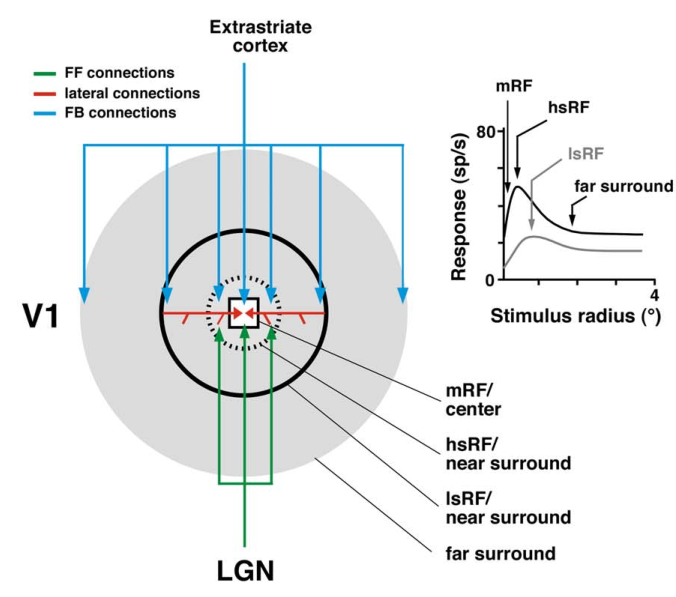
\includegraphics[width=1.0\textwidth]{angelucci_RFstruct.pdf}
	\caption{The receptive field structure of V1 neurons
        showing the minimum receptive field (mRF), high contrast
        summation RF (hsRF) and low contrast summation RF
        (lsRF). Taken from \cite{Angelucci2006}.}
	\label{RFstruct}
\end{figure}

\paragraph{Geniculocortical Afferents and the Minimum and High Contrast Summation RF}

The primary visual cortex receives most of its driving inputs through
the three previously detailed M-, P- and K-cellular geniculocortical
pathways. The M-pathway principally terminates in layers 4C$\alpha$
and 6, the Parvocellular afferents terminate in layers 4A, 4$\beta$
and 6, while K-cells primarily target layer 1 and some regions of
layer 3. By combining anatomical-tract tracing with physiological
recording the spatial extents of feedforward connections have been
measured in detail and linked back to the different RF regions.

The minimum response field as defined above is commensurate to the
classical RF and is usually mapped using drifting gratings masked to a
small disk of optimal parameters for that particular neuron. It is
surrounded by the high contrast summation RF, which is measured by
increasing the size of a drifting grating disk at high contrast until
the neuron reaches its peak response. Using a combination of tracing
and electrophysiological recording \citep{Angelucci2006a} found that
the visuotopic extent of LGN afferents matches the hsRF size of the
target V1 neuron. The diagram and bar chart in Figure \ref{FFmatch}
show how closely the estimates from tracing studies match the results
from physiological classifications of RF areas for magno- and
parvo-cellular pathways. The close match between these different
experiments suggests geniculocortical afferents may underly the extent
of a V1 neuron's mRF. Recent evidence has also shown that the an LGN
neurons hsRF is roughly commensurate with a V1 cell's mRF. This seems
to suggest that the mRF of V1 cells is a product the summation of LGN
cells at their peak spatial summation, while the hsRF region of V1
neurons is defined by the integration of excitatory inputs from
partially suppressed LGN cells. Beyond that it seems likely FF
components partially contribute to surround suppression in V1, however
the spatial scales of surround modulation as well as its orientation
specificity seem to rule out LGN afferents as the major contributor to
the modulatory surround \citep{Angelucci2002,Angelucci2006a}.

\begin{figure}
	\centering
        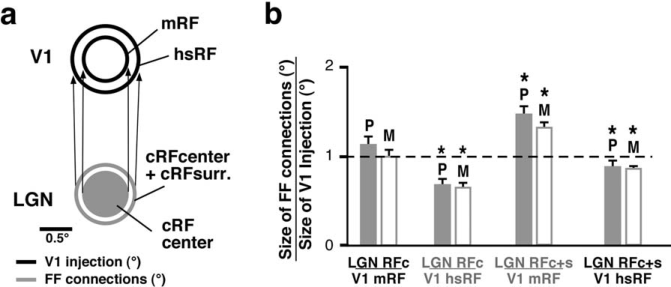
\includegraphics[width=1.0\textwidth]{angelucci_RFmatch.pdf}
	\caption{Comparisons between electrophysiological
        characterisation of RF structure and the spatial structure of
        geniculocortical projections to V1 in (a) diagramatic and (b)
        chart form. Both demonstrate that the mRF and hsRF are
        coextensive with the spatial extents of geniculocortical
        afferents to V1. Taken from \cite{Angelucci2006}.}
	\label{FFmatch}
\end{figure}

Having established the contribution of geniculate afferents to the RF
of V1 neurons its time to look at their spatial distribution. In their
extensive studies and culminating review paper, Angelucci et al.
\cite{Angelucci2006} first fitted the iDOG to the spatial summation
response curve of a number of V1 neurons, injected the recording sites
with tracers and then measured the labeled connections and cell
bodies. The linear extents of the labeled connections were converted
to visual field coordinates using magnification factor (MF) estimates
by \cite{VanEssen1984}. Additionally the anatomic extent of the label
was measured in LGN and again converted to visual space coordinates
using MFs measured by \cite{Connolly1984} and LGN RF size estimates by
\cite{Derrington1984}. These calculations were used to arrive at the
aggregate receptive field (ARF) size, which takes the form:

\begin{equation}
  ARF_{deg} = D^{\degree} + RF_{mean}
\end{equation}

where $RF_{mean}$ is the mean RF size of cells recorded at the edge of
the injection site, which could reflect the mRF, hsRF or lsRF, and
$D^{\degree}$ is defined as:

\begin{equation}
  D^{\degree} = D_{mm} / MF_{mm/deg} + S_{deg}
\end{equation}

where $D_{mm}$ is the diameter, $MF_{mm/deg}$ is the magnification
factor and $S_{deg}$ is the RF scatter at the injection site. The
results show a close match between mRF and hsRF sizes as estimated in
V1 and sizes of the RF center and RF center + surround as measured in
LGN, once again reaffirming the idea that the mRF and hsRF are
primarily driven by geniculocortical afferents. The latest review
\citep{Angelucci2006} has measured the size of the hsRF in V1 neurons
of macaques at 2-8$\degree$ eccentricity as having mean of about
1$\degree \pm$ 0.1, which is roughly 2.2x larger than the mRF of the
same cell based on results from \cite{Angelucci2002} and
\cite{Levitt2002}. Estimates from the latest anatomical study
summarized in table \ref{V1_histology} provides slightly higher
estimates with means of 1.09$\degree$ and 1.41$\degree$ in layer
4C$\alpha$ and 4A/C$\beta$ respectively.

In addition to the spatial extents of V1 RFs, \cite{Angelucci2006a}
also estimated the number of LGN afferents that would contact an
individual V1 neuron. According to their estimates a single neuron in
layer 4C$\alpha$ can be expected to receive roughly 11 projections
from LGN M-cells. Although they were not able to put their own
estimates to the Parvocellular pathway, based on anatomical data from
cats they determined that on average 10 geniculate cells converge on a
V1 layer 4 cell having observed only a maximum of ~30. They conclude
that the geniculocortical pathway in macaques exhibits an even lower
level of convergence than in cats.

In summary, evidence from anatomical and electrophysiological data
seems to suggest that the hsRF of V1 neurons and by proxy the
geniculocortical afferents are on average between 1.0-1.5$\degree$ in
size, exhibiting highly limited convergence with only about 10 cells
targeting a single layer 4 V1 cell.

\paragraph{Lateral Connections and the Low Contrast Summation RF}

Horizontal, lateral or intra-areal connections have been proposed as
the mechanism for a number of observed phenomena, including the
contrast dependence of size tuning, which is why it is thought they
underly the extent of the lsRF. Classically it has been assumed that
lateral connectivity manifests itself through short-range excitatory
and long-range inhibitory connections
\citep{VonderMalsburg1973,Obermayer1990b}. More recent studies have
indicated that intra-laminar projections usually originate in
excitatory pyramidal neurons in layers 2/3, 4B, upper 4C$\alpha$ and
5/6 and at least in layers 2/3 have been shown to target ~80\%
excitatory and ~20\% inhibitory neurons. The spatial scale of these
connections has led several studies to conclude that they may mediate
modulation of RF center properties in the near surround
\citep{Angelucci2002}. Lateral connection could therefore provide a
simultaneous mechanism for a number of observed effects including the
expansion of the summation RF at low stimulus contrast
\citep{Sceniak1999}, colinear facilitation \citep{Mizobe2001} as well
as suppression from the near surround outside the hsRF but within the
lsRF \citep{Sceniak2001,Levitt2002}. The previous section showed that
such phenomena could not be adequately accounted for by
geniculocortical afferents, measurement of spatial extents and
response latencies of horizontal connections reaffirm this view and
have shown that the lsRF and lateral connections are coextensive
\citep{Angelucci2002}.

Apart from the exact spatial dimensions of horizontal connections, it
is important several other functionally important properties. While
layer 2/3 neurons display patchy connectivity, linking regions with
similar functional properties such as orientation preference or ocular
dominance, this has been shown not to be the case in macaque layer 4B,
upper 4C$\alpha$ \citep{Angelucci2002}. In addition, it was found that
horizontal connections in macaque V1 are isotropic in visual space
unlike the anisotropy along the axis of preferred orientation observed
in tree shrews \citep{Bosking1997} and several other species. This may
also indicate that contour completion in macaques is mediated by
feedback connections. Horizontal connections have been shown to
illicit only subthreshold responses \citep{Hirsch1991} and are thus
limited to modulatory influence. However, as the surround modulation
extends far beyond the monosynaptic spread of lateral connections it
is unlikely they account for modulation from the far
surround. Polysynaptic chains of lateral connections are also an
unlikely substrate for the far surround due to the slow conduction
velocity of their axons. In particular, \cite{Bair2003} showed that
onset latencies of suppression from the far surround were almost equal
to the delays from the near surround. This makes it likely that far
surround modulation is mediated primarily by inter-areal feedback
connections, which we will look at in detail at a later stage.

Having established that spatial profile of lateral connections is
commensurate to that of the lsRF and vice versa the data from both
sources will be laid out and analyzed. Anatomic data suggests that the
spatial spread of lateral connections can be anywhere between 3-10 mm
(on average 6-7 mm) in total length \citep{Angelucci2002}, which is
broken down by layer in table \ref{LatExtents}. Along its principal
axis the visuotopic monosynaptic spread of V1 horizontal connections
has a mean of $2.47\degree \pm 0.3\degree$. This falls well within the
range of estimates for the lsRF as published in a number of studies
\citep{Shushruth2009,Sceniak1999,Sceniak2001}, which were fit with the
same integrated DoG model and stimulus protocol as used in the
\cite{Sceniak2006} paper on the spatial properties of LGN neurons,
reviewed previously.

In summary, there is strong evidence that lateral connections underly
the extent of the lsRF and mediate a number of effects in the near
surround, including contrast dependent size tuning, colinear
facilitation and low contrast suppression. Unlike in other species
horizontal connections are isotropic but do exhibit patchy
connectivity in layer 2/3. The extents of horizontal connections range
between 3-10 mm, which averages to around 2.5$\degree$ in visual
space.

\begin{table}
\centering
\begin{tabular}{l | c c}
  \hline \hline Cortical Layer & Mean $\pm$ SD & Range \\ \hline 2/3
  ($n = 10$) & 6 $\pm$ 0.7 & 3-9 \\ 4B/4C$\alpha$ ($n = 8$) & 6.7
  $\pm$ 0.7 & 4.7-10 \\ 5/6 & 7.9 $\pm$ 1.6 & 6.3-9.5 \\ \hline
\end{tabular}
\caption{Extents of macaque V1
lateral connections between 2.5-7.5$\degree$ eccentricity broken down
by layer given as $D_{mm}$ along V1's elevation axis. Taken from
\cite{Angelucci2002}.}
\label{LatExtents}
\end{table}

\paragraph{Feedback from Higher Cortical Areas and the Far Surround}

As the previous to sections have shown, modulatory influences to V1
RFs extend well beyond the spatial spread of both geniculocortical
afferents and horizontal connections. This extended modulatory field
is known as the far surround and is thought to be mediated by feedback
from higher cortical areas. The far surround has generally been
characterized as suppressive, especially for iso-oriented gratings in
the center and far surround. More detailed analysis has shown that the
far surround can also exhibit response facilitation under some
stimulus conditions. This section will characterize the function,
termination patterns and spatial extents of feedback connections from
higher cortical areas to V1.

The notion of a hierarchical organization of cortical visual areas has
been around for quite some time and more recent analysis of
feedforward and feedback connections has affirmed this view. At the
bottom of this hierarchy is V1, sending partially segregated FF
projection to areas V2, V3, V4 and visual area middle temporal (MT),
which all send FB projections back to V1
\citep{Felleman1991}. Feedforward projection from V1 to V2 arise
mainly from layer 4B and to a lesser degree from layer 2/3 and
6. Feedback connections on the other hand arise from layers 2/3A and
5/6 and terminate in the same layers from which FF connections are
sent, which means the cells projecting up the hierarchy often overlap
with the termination regions of FB projections being sent back down
\citep{Angelucci2002}.

Just like lateral connections FB connections do not drive their target
cells, exhibiting only modulatory influence on the RF center
\citep{Bullier2001a}. Inactivation of areas V2 and MT has been shown
to reduce the firing rate of V1 neurons to stimuli in their RF center
\citep{Hupe1998}, suggesting FB inputs are summed with FF inputs to
increase activity. The exact balance between excitation and inhibition
of FB connections is so far not very well explored in macaques but
evidence from rats suggest that they almost exclusively target
excitatory cells. However \cite{Angelucci2006} and \cite{Schwabe2006}
have proposed a regimen where FB connections in the far surround
target pyramidal neurons, which in turn send monosynaptic horizontal
connections to excitatory and inhibitory neurons in the RF center and
can thus mediate both suppressive and facilitatory effects depending
on stimulus properties.

Feedback connections have been thought to underly a number of top-down
effects in V1, including attention \citep{Treue2003}, the reverse
hierarchy theory of visual learning \citep{Ahissar2004} but more
recent studies have suggested they contribute directly to the response
of V1 neurons to simple visual patterns
\citep{Angelucci2002,Angelucci2003,Schwabe2006}. Notably
\cite{Schwabe2006} and \cite{Ichida2007} seem to have resolved the
conflicting evidence about the far surrounds suppressive and
facilitatory role. Using both experimental and theoretical work they
found that while the far surround is suppressive under high contrast
conditions, the response of a neuron to a low contrast stimulus in the
RF center is facilitated by a small annular stimulus in the far
surround. This indicates that excitatory and inhibitory surround
mechanisms have similar extents and that the sign of their
contribution depends on changes in local excitation/inhibition balance
brought about by surround stimulation.

The spatial and functional organization of the FB pathway is thought
to differ significantly from FF connections. They seem to exhibit less
precise retinotopic organization and terminate in a more diffuse
fashion than FF connections. However, more recent evidence suggests
that at least a subset of FB connections exhibit patchy and
functionally specific termination patterns
\citep{Angelucci2006}. Evidence from new world primates has also shown
that V2 FB axons to V1 link regions of similar orientation preference
and that their terminal fields are anisotropic along the axis of the
preferred orientation of the originating cell in V2
\citep{Shmuel2005}. The discrepancy between different studies in
finding diffuse and patchy FB termination patterns may be attributable
to different labeling methods and given that CTB labeling is the more
mature and tested procedure it seems likely that FB connections do
exhibit patchy terminations in layers 1B, 2/3, 4B and 5/6 and diffuse
terminals in layer 1A. The observation of patchy connectivity is also
consistent with their proposed functional role in mediating
feature-specific influences from the far surround.

The anatomical spatial extents of FB connections from higher cortical
areas have been measured in a number of tracing
studies. \cite{Angelucci2002} provides a measurements broken down by
area, measuring the extents of FB connections from V2, V3 and MT to V1
(see table \ref{FBExtents}). Once converted into degrees of visual
space the results are the following: Feedback from V2 has a mean size
of 3.4$\degree$ in layer 2/3 and 3.8$\degree$ in layers 5/6, FB from
V3 a mean size of 5.6$\degree$ in layers 2/3 and 6.7$\degree$ and FB
from MT a mean size of 15.3$\degree$ and 26.6$\degree$ in the upper
and lower layers respectively. The largest far surround field measured
was 28$\degree$ in diameter and the measurement was still limited by
the maximal presented stimulus size \citep{Ichida2007}. These results
clearly indicate that cortical feedback to V1 increases in its spatial
extents and becomes less spatially and retinotopically specific when
moving up in the cortical hierarchy to the point where it covers huge
portions of the visual field.

Feedback projection from higher cortical areas to V1 mediate a number
of important contextual effects and has been implicated in the early
stages of visual attention but also seem to be closely involved in the
processing of simple visual stimuli. This section has summarized
current knowledge on the spatial termination patterns of FB
connections to V1, indicating how they could give rise to functional
properties of V1 information processing. While this information will
aid the development of a strongly constrained model, without an
understanding of the information content being fed back to V1 from
higher cortical areas understanding of their true function will be
limited.

\section{The Internal Circuitry of Striate Cortex}

The previous section outlined the overall structure of the early visual
system, breaking down the contribution of inputs from various sources
on the receptive field (RF) of neurons in primary visual cortex
(V1). While this provides general anatomical constraints and sheds
some light on the functional circuitry underlying many of the
contextual effects that have been observed in the primary visual
cortex, it does not address many of the fundamental questions about
the functional significance of recurrent cortical processing. In
particular, it does not address the delicate balance in both strength
and spatial extent between excitation and inhibition that is required
to halt runaway excitation, sparsify the inputs and thereby allow for
the formation of concentrated activity bubbles around which
self-organization can take place. This section will cover how the
understanding of intra-cortical connectivity has evolved and how this
has been reflected in various developmental and non-developmental
models.

\subsection{The Mexican Hat}

Before complex tracing and circuit reconstruction techniques became
available, considerations about the connectivity profiles in the
cortex were largely theoretical or based on data from other anatomical
structures, which were at the time more amenable to study. Anatomical
data and electrophysiological studies in the retina had shown that
there is a strong lateral inhibitory component involved in
decorrelating photoreceptor activities, thereby enabling more
efficient coding of the input \citep{Atick1992}. Lateral inhibition
was taken to be a general principle of sensory systems and, among
others, \cite{Blakemore1970} suggested repulsive interactions between
neighboring contours could account for psychophysical data. Further
evidence of lateral inhibition as a general feature of sensory systems
was provided by a variety of theoretical models of self-organization,
highlighting the necessity of effective local excitatory and long
range inhibitory interactions for the formation of local activity
bubbles, which in turn provided the basis for orderly map organization
\citep{VonderMalsburg1973,Miller1989}.

The connectivity profile employed in the various self-organizing map
models became known as the Mexican hat profile due to its strong
resemblance to a sombrero. A simulated Mexican hat profile is shown in
\ref{MexHat} generated through a simple difference of Gaussian (DoG),
whereby a small positive Gaussian kernel is combined with a larger
inhibitory kernel. A large variety of cortical models have
successfully employed this connection profile to explain a variety of
effects ranging from topographic map organization, orientation tuning
and contextual effects. Problematically, it is unclear how
biologically realistic the assumption of strong local excitation and
broadly tuned or untuned inhibition is.

\begin{figure}
	\centering 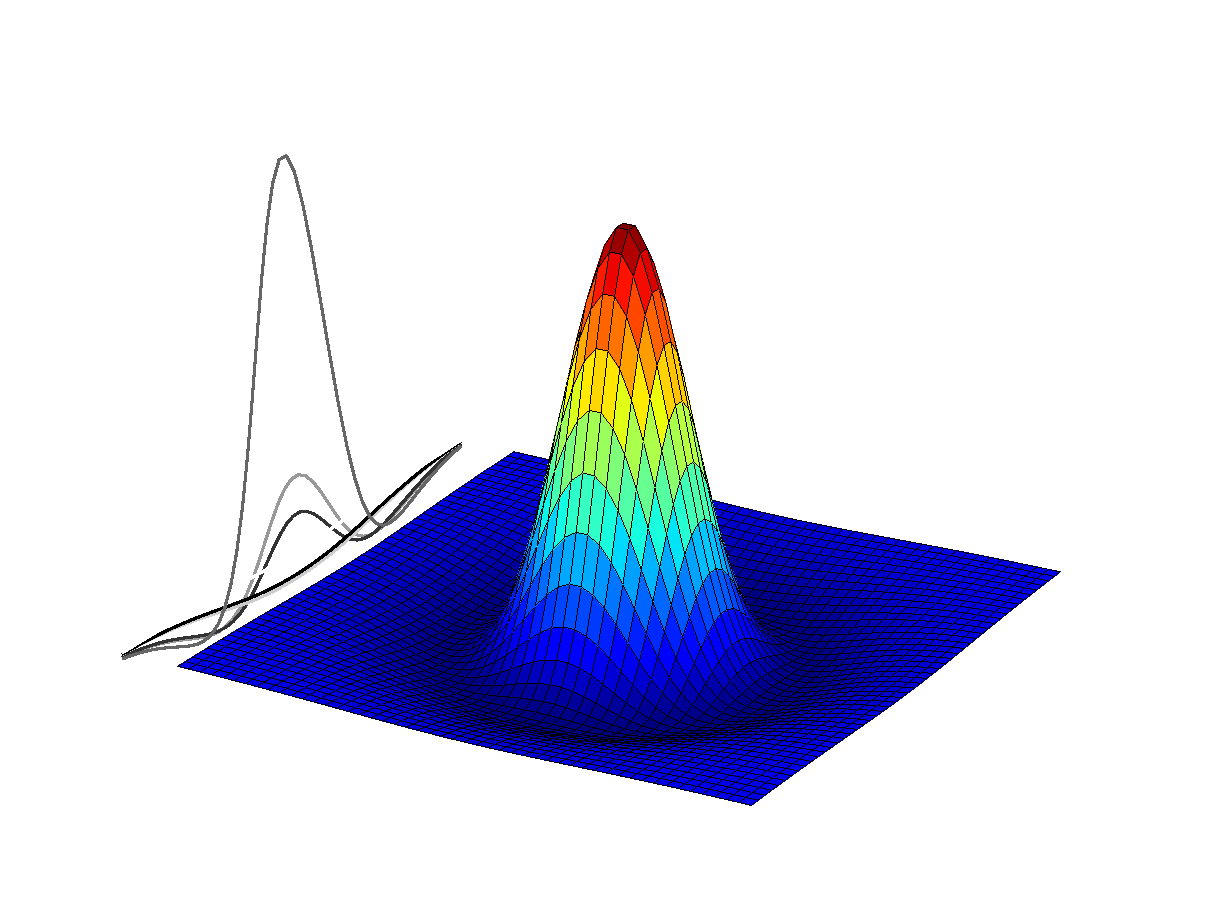
\includegraphics[width=0.7\textwidth]{mexhat.pdf}
	\caption{3D plot of
        Mexican Hat connectivity.}
	\label{MexHat}
\end{figure}

Since then a number of lines of evidence have come together to show
that this spatial connectivity profile does indeed seem to exist, at
least when considering the aggregate circuit under certain stimulus
conditions. Electrophysiological and optical imaging have both
confirmed that strongly driven cortical neurons receive strong local
excitation and long-range lateral inhibition
\citep{Grinvald1994,Sceniak2001}. At high contrasts
\cite{Grinvald1994} showed that a neuron responding to a small,
central grating stimulus in isolation exhibits far greater levels of
activity than when presented with a co-linear surround stimulus
alongside the central stimulus. This highlights an interaction between
the center and surround RF that is not only dependent on the
orientation statistics but also on the contrast levels in the
input. In particular \cite{Hirsch1991} and \cite{Weliky1995} showed
that lateral connections impinging onto a neuron would exert a small
excitatory effect, when embedded in a low contrast surround, while
high contrast would flip the sign of these contextual influences and
suppress the central neurons activity. Additionally, \cite{Hirsch1991}
found that laterally evoked EPSPs, presumably underlying facilitatory
effects, experienced strong voltage-dependent enhancement, speculating
that this would allow stimuli in the surround to modulate cRF
responses without driving the response on its own.  This provides
functional evidence that the aggregate circuit can produce a Mexican
hat profile under the right stimulus conditions but also suggests that
the underlying circuitry is more complex.

Precisely how these two input-dependent modes of contextual
integration emerge is unclear. However, as anatomical tracing
techniques have become more sophisticated and biomarkers for different
cell types were discovered, attempts have been made at teasing apart
the cortical circuit. These anatomical surveys showed that long-range
connections extending beyond a single orientation column were almost
exclusively excitatory and 80\% of these excitatory synapses target
other excitatory pyramidal neurons
\citep{Hirsch1991,Kisvarday1997a}. The remainder of these connections
were shown to target inhibitory interneurons, which would in turn
contact pyramidal neurons, suggesting a di- or poly-synaptic mechanism
for long range suppression. On the basis of some of this work
\cite{Douglas1991} developed what has become known as the canonical
microcircuit for the neocortex. This circuit includes separate
inhibitory and excitatory neurons, which are driven by thalamic
afferents and recurrent connections. Further work has fleshed out the
spatial profiles of these connections, which ultimately gave rise to
the simplified circuit described in Figure \ref{V1MicroCircuit}. This
goes some way toward reconciling anatomy with the experimentally
measured functional connectivity profile at high contrast levels.

\begin{figure}
	\centering
        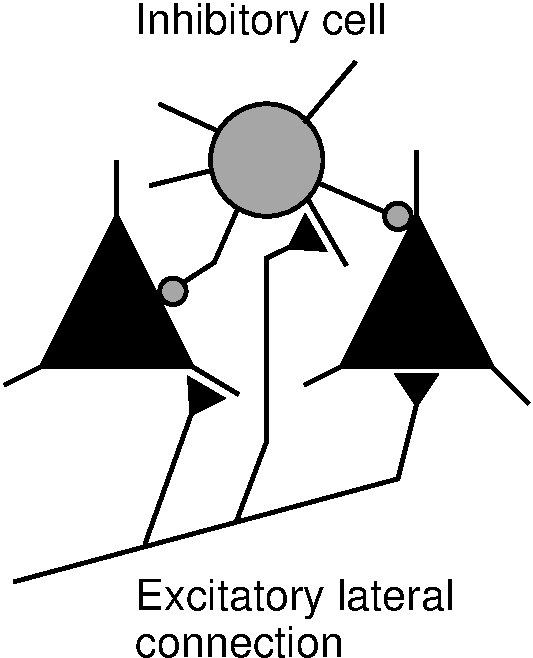
\includegraphics[width=0.25\textwidth]{weliky_microcircuit.pdf}
	\caption{Local microcircuit for long-range suppression through
          di- or poly-synaptic circuit in V1. Reproduced from
          \cite{Miikkulainen2005b} as adapted from \cite{Weliky1995}.}
	\label{V1MicroCircuit}
\end{figure}

More recent attempts at reconciling anatomy with function have been
able to further resolve some of the problem. In particular, there is
clear evidence showing that excitatory synapses onto excitatory and
inhibitory neurons differentially target their recipient
neurons. Excitatory connection onto inhibitory interneurons seem to
preferentially synapse perisomatically, in contrast with recurrent
long-range excitatory connections which have been shown to target
their recipient neurons dendritically
\citep{Gilbert1990,McGuire1991}. Additionally, at least a subset of
inhibitory interneurons seem to preferentially target the soma of
pyramidal and stellate cells they inhibit \citep{Markram2004}. On that
basis it is reasonable to assume that inhibitory connections are, in
general, stronger and may act divisively.

Although these divergent properties of excitatory and inhibitory
neurons were only discovered recently it had long been proposed that
inhibitory interneurons are inherently more effective at suppressing
activity than recurrent excitatory connections are at exciting the
network, but due to a high threshold or some other related mechanism
the inhibitory neurons are not strongly recruited unless there is
strong afferent input \citep{Sillito1979}, as would be the case under
high contrast conditions. Although it is now clear that network
effects allow for strong long-range inhibition through di- or
poly-synaptic connections under the right stimulus conditions, the
mechanisms by which contrast dependent behaviors emerge from the
cortical circuit are still only vaguely characterized.

A number of models have been developed to explain contrast dependence
of contextual effects on the basis of the general principle of
asymmetry between the response properties of excitatory and inhibitory
neurons. One of the first to publish such a model were
\cite{Stemmler1995}, who suggested inhibitory neurons require higher
external input rates before activating because they receive
significantly less spontaneous background input as compared to
excitatory neurons, an effect known as stochastic resonance. Although
this mechanism has at least been theoretically reaffirmed
\citep{Bezrukov1997}, there is no experimental data establishing it as
a functionally significant mechanism in V1. Other models, hoping to
account for a wider array of RF effects implement such a mechanism
directly by setting a higher threshold in the inhibitory population
and introducing very strong lateral excitation of inhibitory neurons
\citep{Schwabe2006}. Another suggestion was made by \cite{Somers1998},
who in addition to a simple threshold asymmetry, also point to the
claim by \cite{Thomson1994} and others \citep{Abbott1997,Tsodyks1997},
that synaptic depression causes recurrent excitation to quickly
decline in efficacy during high frequency stimulation, while
facilitation of excitatory synapses onto inhibitory interneurons
increases transmission efficacy as presynaptic firing rates increase
\citep{Thomson1995}. The suggestion that inhibitory neurons have a
higher contrast threshold has become very popular in the theoretical
literature of the past 20 years, however as of yet there is only
limited evidence to support this core assumption and there are a
number of alternative or concurrent mechanisms that may explain all or
at least some of the contrast dependent effects.

%% Before looking in more detail at the effects and mechanisms of surround suppression it is important to consider what the functional significance the excitatory and inhibitory components have in the circuit. \cite{Douglas1995} looked at precisely this problem by taking a network level approach on the basis of which they were able to draw several conclusions. By considering excitatory and inhibitory feedback as time-dependent network conductances, they concluded that as a noisy input signal is presented to a orientation selective V1 population, the network determined gain of individual neurons would at first be almost equal, would then be averaged by the inhibitory interneurons, which in turn provide an effective threshold for the pyramidal cells. As pyramidal neurons fall silent, due to an iceberg effect, the effective gain between the surviving pyramidals increases, amplifying the remaining signal. Through such a process of variable thresholding and amplification, a network could restore incomplete and noisy inputs based on the statistics stored within its lateral connectivity. In such a scenario, the rate of decay of the surviving neuron ensemble is effectively slowed leading to selective amplification.

As the last paragraphs have shown, inhibition and in particular
surround inhibition are at the core of the major discussions on
contrast dependent effects and surround modulation and a more thorough
understanding of the spatial, temporal and functional dynamics of
surround inhibition is required.

\subsection{Surround Suppression: Feedforward or Feedback?}

The last section highlighted how little we still know about the origin
of surround suppression and inhibition. There is still significant
controversy whether surround suppression originates in feedforward or
feedback pathways or whether both contribute over different spatial
scales. This includes suggestions that surround suppression in the
classical RF are mediated through synaptic depression in the
thalamo-cortical afferents \citep{Carandini2002}, broadly tuned
inhibition by thalamo-cortical recipients, long-range excitation of
local inhibitory interneurons or even through various feedback
mechanisms. This section will detail the evidence for each of these
proposals, the possibly anatomical origin of each of these mechanisms
and tease apart the circuit by looking at interactions between
surround suppression, stimulus size and contrast.

Since the circuitry of the cortex is so complex, the task of
segregating feedforward and feedback contributions to surround
suppression is highly difficult. Although only a starting point, one
way of starting to tease these two possible contributions apart is to
look at the time course of suppression. In the literature early and
late components to surround suppression have been identified. The
early component is characterized as being driven by lower CRF
contrasts with spatio-temporally broad band tuning and little
adaptation \citep{Levitt1997,Cavanaugh2002a}. The late component on
the other hand is driven more strongly by high contrast stimuli in the
CRF, has sharp spatio-temporal tuning and can be strongly affected by
adaption \citep{Levitt1997}. Evidence suggests that the early, broadly
tuned component originates in the LGN and the thalamocortical
recipient layer of visual cortex \citep{Blasdel1984a,Hawken1996}. In
monkey cortex in particular, this broadly tuned suppressive effect is
only weakly evident in the LGN and is thought to arise much more
strongly in layer 4 of striate cortex \citep{Webb2005}, which may have
some correspondence to the broadly tuned inhibitory population
identified by \cite{Hirsch2003}. \cite{Carandini2002} on the other
hand suggest that there is a synaptic explanation for surround
suppression, primarily due to the speed with which the suppression
arrives, its immunity to cortical adaptation and the fact that it is
restricted to the CRF. However, they concede that synaptic depression
doesn't account for gain control and the abolishment of
cross-orientation suppression by GABA$^{A}$ blockade, so a mechanism
that can account for all these phenomena may still be preferable. In
that vein, \cite{Webb2005} propose two inhibitory mechanism one of
which sums local activity in a neurons CRF and divides the response of
the CRF and the later component that receives inputs from a much
larger area but provides narrowly tuned suppression. The broadly tuned
component in particular has a strong relationship with contrast gain
control, which has been firmly established to act
divisively. Independent work by \cite{Xing2005} supports the
suggestion of two inhibitory components and further expand on the size
dependence of these two components. Specifically, they conclude that
the tuned component is recruited far more strongly for larger stimuli,
which seems to confirm a contribution from beyond the CRF.

This recent work has identified two clear and distinct inhibitory
components but have not yet fully described which mechanisms and
circuits they are mediated by, the next section will attempt to
address this shortcoming.

\subsection{Distinct Inhibitory Populations}

In order to begin teasing apart the origin of intracortical surround
suppression mediated by local inhibitory circuits it is necessary to
consider the different candidate cell classes. While there are a long
list of different inhibitory cell types based on their morphology and
spiking behavior, recent techniques have divided inhibitory into
several broad, functionally distinct classes based on their
immunoreactivity. The two cell types considered here are parvalbumin
(Pv-ir) and somatostatin (Sst-ir) immunoreactive neurons, which are
primarily differentiated by the cellular locus of their synaptic
targets. While Pv-ir neurons seem to target pyramidal cells
perisomatically, Sst-ir neurons target their recipients
dendritically. The following subsections will detail the anatomical,
physiological and functional differences between these cell classes.

\subsubsection{Parvalbumin Immunoreactive cells}

The two main cell types, which exhibit parvalbumin immunoreactivity
are the chandelier and basket cells \citep{Binzegger2004}. While
chandelier cells make up only a small fraction of GABAergic neurons in
the cortex and are primarily found in layer 2/3, the fast-spiking (FS)
basket cells are the predominant interneuron subtype in the mammalian
cortex across all lamina, accounting for 42\% in layer 2/3 and layer 5
and 78\% in layer 4 of the cat \citep{Hogan1992,Huxlin2001} and up to
74\% across cortical layers in macaque \citep{VanBrederode1990}. The
abundance in the thalamocortical recipient layers and the fact that
they preferentially target the soma and proximal dendrites of spiny
neurons with multiple strong synapses, exhibiting high probability of
GABA release \citep{Freund2007,Markram2004}, ensures basket cells are
of tremendous interest. On that basis it has been suggested that the
perisomatic connectivity profile of basket cells gives them the
ability to provide shunting inhibition to layer 4 spiny neurons,
acting divisively to control their response gain \citep{Wilson2012}.

Basket cells can be further subdivided, primarily based on their size,
into clutch and large basket cells. However all basket cells can make
multiple connections onto a target pyramidal neuron
\citep{Somogyi1983} and have a considerable spatial extent
\citep{Kisvarday2002}. In particular, studies in cat area 17 and
macaque V1 have identified basket cells 1-2 mm in extent
\citep{Somogyi1983,Lund1987,Lund1991,Martin1983} and single cell
tracing studies have even identified large basket cells, which give
off a roughly uniform number of boutons across a large diameter
spanning up to two hypercolumns \citep{Buzas2001}. A schematic
representation of the basket cell connectivity profile is summarized
and compared against both the orientation column structure and the
excitatory connection profile in Figure
\ref{BasketCellExtent}. Functionally such a connectivity profile may
indicate that basket cells can suppress neurons with widely varying
orientation, which may implicate basket cells as an important
mechanism to sharpen orientation preference.

\begin{figure}
	\centering
        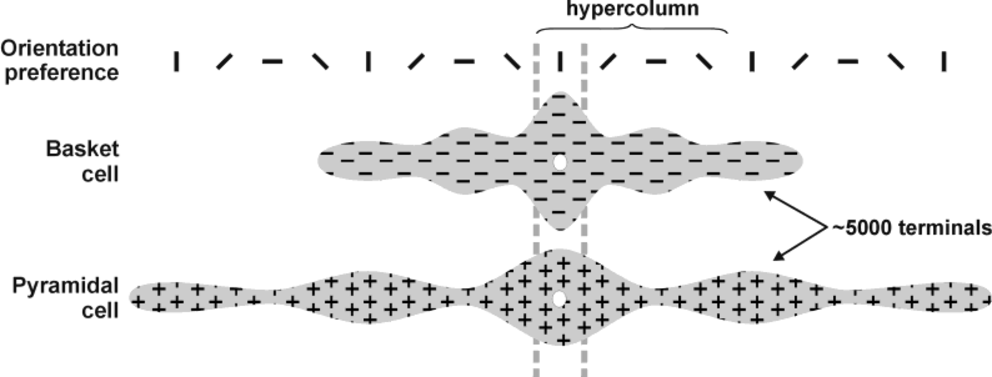
\includegraphics[width=1.0\textwidth]{basketcellextent.pdf}
	\caption{Summary schematic comparing relationship between
        long-range basket cell and excitatory connectivity with the
        underlying orientation preference structure. Upper legend
        represents different orientation domains in the cortical
        topographic map. Grey dotted lines indicate the orientation
        column within which soma of the simplified basket cell and
        excitatory neuron are found. The grey field with minus signs
        indicates the extent of inhibition provided by the basket cell
        connections considered in the current study. The grey region
        with plus signs indicates the excitatory field of a
        stereotypical pyramidal cell based on previous data by
        \cite{Bosking1997,Kisvarday1997a} and others. The height of
        the grey plus/minus regions indicates the number of axon
        terminals provided in that column. While basket cell terminals
        show local maxima every half hypercolumn distance, pyramidal
        cell terminals are maximal at every full hypercolumn
        distance. Reproduced from \cite{Buzas2001}.}
	\label{BasketCellExtent}
\end{figure}

In terms of their spiking behavior Pv-ir cells are characterized as
being fast fast-spiking (FS) neurons, often firing in bursts with a
very short response latency. Further, evidence from somatosensory
cortex in rodent and lagomorph species suggests they receive strong
input from thalamocortical afferents arriving in layer 4 and very
effectively suppress sustained firing from spiny neurons receiving
inputs from the thalamus \citep{Swadlow2003}, implicating them in
feedforward inhibition. This feedforward inhibition circuit is shown
in Figure \ref{burkhalterpv}. Their effectiveness in suppressing
feedforward activity can be explained by the large number of
thalamocortical axons they receive, which exhibit faster kinetics than
those targeting spiny neurons \citep{Cruikshank2007,Gabernet2005}, and
the fact that they evoke large inhibitory responses in spiny cells
\citep{Cruikshank2007,Gabernet2005}.

It is also important to note that the thalamocortical synapses onto
the Pv-ir population have been shown to be depressed by repetitive
activation, resulting in weaker feedforward inhibition at high
stimulation frequencies \citep{Gabernet2005}, a property which may
indicate lower activation of the PV population at high contrasts. The
Pv-ir population may also play an important role in network
homeostasis as activity blockade has been shown to decrease the
efficacy of Pv-ir inhibition \citep{Bartley2008}, thereby indirectly
up-regulating activity in excitatory cells. Further, selectively
up-regulating Pv-ir cells using optogenetic stimulation was shown to
have a similar effect as lowering the contrast, which is to increase
preferred size and weakening surround suppression
\citep{Nienborg2013}. This is compatible with the idea that Pv-ir
neurons provide strong feedforward inhibition such that the input
drive in the cortex is decreased, as would be observed under low
contrast conditions. Overall then, Pv-ir neurons show strong
interaction with stimulus contrast and may be involved in regulating
the gain of the network with complex implications for the contrast
response of the network.

\begin{figure}
	\centering
        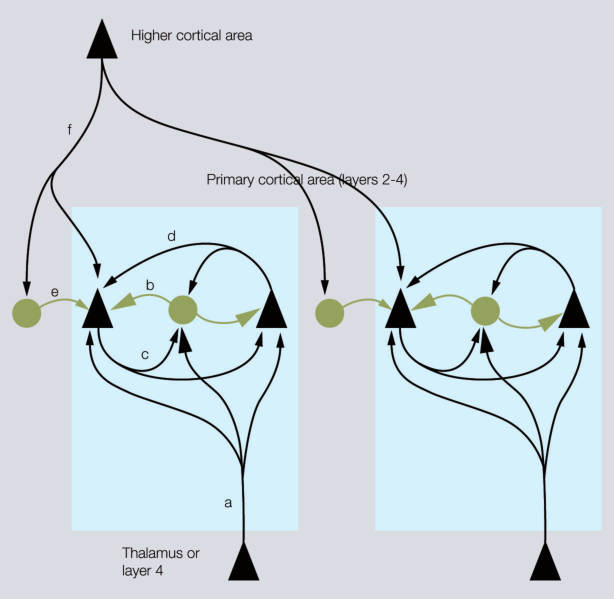
\includegraphics[width=1.0\textwidth]{burkhalter_pv.pdf}
	\caption{Inhibitory networks involving fast-spiking
        parvalbumin-immunoreactive neurons in thalamocortical,
        interlaminar and interareal cortical circuits. Feedforward
        excitatory thalamocortical inputs to pyramidal cells, spiny
        stellate neurons ($\blacktriangle$) and fast spiking
        interneurons ($\newmoon$) in layers 2-4 (a). Inputs to
        interneurons are stronger (large arrowheads) than inputs to
        spiny cells. PV neurons provide strong (large rectangular
        endings) feedforward inhibition (b) to spiny cells. Feedback
        inhibition (c) results from PV neurons that are excited by the
        same spiny neurons that they inhibit. These reciprocally
        connected spiny neuron/PV neuron pairs share common inputs
        (e.g., cells in layer 4 from thalamus or cells in layer 2/3
        from layer 4) creating recurrent excitatory (d) and inhibitory
        subnetworks (contained within blue shaded boxes). ‘Lateral’
        inhibition (e) of these subnetworks results from PV neurons
        that are driven by excitatory feedback connections (f) from
        outside the subnetworks (e.g., by layer 5 to layer 2/3
        connections or feedback from higher cortical areas). Notice
        that ‘lateral’ inhibition is weaker (small rectangular
        endings) than feedforward and feedback inhibition and impinges
        on multiple subnetworks. Reproduced from
        \cite{Burkhalter2008}.}
	\label{burkhalterpv}
\end{figure}

There is still considerable debate on the extent to which this
subpopulation is tuned to a particular orientation. Most
visuo-cortical models employ broad, non-specific GABAergic inhibition
\citep{Somers1998,Troyer1998}. This seems to be supported by
anatomical evidence, which has long shown that inhibitory projections
are generally diffuse and display low specificity for specific
stimulus features \citep{Albus1994,Kisvarday1997a}. Further,
electrophysiological data paints a similar picture, revealing
suppression that is broadly tuned for stimulus attributes, providing
orientation unspecific suppression from a visual region that is
coextensive with the classical RF \citep{DeAngelis1992}. Recent
attempts at studying the Pv-ir neurons at the single neuron level have
revealed a mixed picture. While the cells as a whole were broadly
tuned to various stimulus features, individual branches often
displayed very high specificity, which may underlie subfield
antagonism and contribute to a push-pull configuration
\citep{Kisvarday2002}. Studies in mouse visual cortex seem to confirm
such a dual purpose of Pv-ir neurons, although they also find higher
heterogeneity in the Pv-ir population \citep{Runyan2010}. This may
indicate a laminar differentiation in function as studies of Pv-ir
neurons in the thalamocortical recipient layer 4 have characterized
them to exhibit very broad tuning, due to their low spiking threshold
and more convergent inputs \citep{Ma2011}. However, even in layer 2/3
most Pv-ir cells displayed broad orientation tuning
\citep{Hofer2011}. Further studies in cat area 17 find very similar
results identifying a class of inhibitory complex cells in layer 4
exhibiting weak orientation tuning \citep{Hirsch2003}, which can
primarily be accounted for by the tuning of synaptic responses and a
lower spike threshold \citep{Nowak2008}. A more recent study in
auditory cortex seems to affirm these conclusions, hypothesizing that
`while PV neurons may provide broadly tuned feedforward inhibition for
a rapid control of ascending inputs to excitatory neurons, the delayed
and more selective inhibition from SOM neurons may provide a specific
modulation of feedback inputs on their distal dendrites`
\citep{Li2014}. Further study will be needed to confirm whether these
results extend to the primate, however it is clear that basket cells
generally display weaker tuning than spiny neurons in V1.

Based on our current knowledge of Pv-ir cell population and more
specifically the basket cells, it is clear that they provide a good
candidate mechanism to account for a number of phenomena. Their fast
response profile, large spatial extent and the relative weakness in
their orientation tuning may allow them to carry out fast, adaptive
gain control, broadly tuned suppression and thereby sharpen the
orientation preference of the PNs in their vicinity. So while synaptic
depression may still provide an alternative explanation for many of
these phenomena, it is likely that the Pv-ir population carries out at
least some of these functions.

\subsubsection{Somatostatin Immunoreactive cells}

The Sst-ir population has been characterized to a lesser extent, but a
general consensus is beginning to emerge around their function and
electrophysiological properties. The Sst-ir cells account for around
half of the non-PV-expressing neurons \citep{Gonchar2007,Xu2010} and
preferentially synapse onto distal dendrites and dendritic tufts of
pyramidal neurons \citep{DiCristo2004,Silberberg2007}, on the basis of
which it has been suggested that Sst-ir neurons act subtractively
\citep{Wilson2012}.

In trying to characterize the excitatory inputs to Sst-ir cells in
layer 2/3 of the mouse, \cite{Xu2009} determined that unlike Pv-irs,
the main source of excitation of Sst-irs were horizontal axons within
layer 2/3 not the ascending layer 4 axons. This property also
contributed to the size dependent responses of the Sst-irs, which were
shown to be recruited progressively more strongly when they were
exposed to optogenetic photostimulation of increasing
diameter. Importantly, the Sst-ir response grew larger even when
photostimulation reached beyond its maximal dendritic extent,
demonstrating that the recruitment of increasingly more distant
pyramidal cells provided their main excitatory drive. This putative
circuit is shown in Figure \ref{som}, exhibiting their pooling of
tuned, excitatory input from pyramidal cells across a large area,
providing only very local inhibition. Additionally it seems that
Sst-ir interneurons are capable of disinhibiting the thalamocortical
recipient layer 4 by targeting Pv-ir cells \citep{Xu2013}.

In terms of their response properties the Sst-ir neurons have been
shown to exhibit much lower levels of spontaneous and evoked activity,
stronger orientation and direction selectivity and longer response
latencies than Pv-ir neurons in mouse visual cortex
\citep{Ma2011}. These properties are consistent across both layer 2/3
and 4 and may point to a role in gating later arriving intracortical
excitatory inputs. In terms of their tuning properties Sst-ir neurons
display smaller On/Off subfields with less overlap than nearby spiny
neurons and orientation tuning on par with pyramidal neurons. While
most data on their tuning properties comes from rodent visual cortex,
which does not exhibit a topographic organization of orientation
tuning, it seems the stronger orientation selectivity of Sst-ir cells
can be accounted for by their preferential connectivity to neurons
with similar orientation preference as well as a higher spiking
threshold and weaker excitatory inputs \citep{Bartley2008}. Another
interesting feature of Sst-ir response properties is the fact that
although their excitatory inputs are weak, they are facilitating
resulting in delayed but strong activation under high frequency
stimulation \citep{Beierlein2003,Bartley2008,Tan2008}. Based on these
properties, Sst-ir neurons would only be recruited to provide
significant inhibition if the stimulus contrast or size reaches a
certain level \citep{Adesnik2012}. Thus they could provide a direct
mechanism for contrast dependent size tuning and surround modulation
effects, being only weakly recruited when contrast or stimulus size is
low but becoming strongly activated at higher contrast levels and for
larger stimulus sizes.

% Comment on difference between high threshold and Sst-ir cell hypothesis

Another suggested role for Sst-ir neurons is the gating of feedback
signals on the distal dendrites of principal neurons. The Martinotti
cells, which provide strong axonal projections to layer 1 of the
cortex, make up a large proportion of Sst-ir neurons in layer 2/3 of
the cortex and are therefore well placed to suppress feedback signals
arriving in the superficial layers of the cortex
\citep{Fanselow2008,Gentet2012}. In the rodent somatosensory cortex,
\cite{Gentet2012} showed that Sst-irs in layer 2/3 become
spontaneously active during passive wakefulness but are strongly
suppressed during active whisking behavior, presumably by the
vasoactive intestinal peptide (Vip)-ir population. The Sst-ir cells
may therefore be involved in mediating top-down control of sensory
processing, effectively gating context-dependent processing in a state
dependent manner.

\begin{figure}
	\centering
        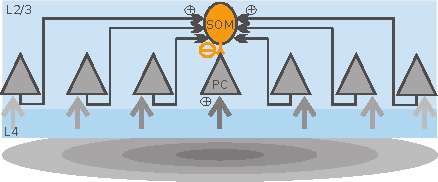
\includegraphics[width=1.0\textwidth]{adesnik_som.pdf}
	\caption{Schematic illustration of the cortical circuit in
          layer 2/3 contributing to surround suppression. As a visual
          stimulus expands (larger stimuli are shown in lighter grey),
          recruitment of adjacent PCs increases Sst-ir excitation
          through horizontal axons (horizontal arrows). Reproduced
          from \cite{Adesnik2012}.}
	\label{som}
\end{figure}

In summary, Sst-ir neurons seem to provide delayed and
feature-selective feedback inhibition, which puts them in a good
position to effectively gate late arriving intracortical excitatory
inputs arriving from either lateral or feedback connections but may
also be implicated in suppressing feedforward inhibition by
inactivating layer 4 Pv-ir cells.

\subsubsection{Vasointestinal peptide expressing interneurons}

The previous review focused primarily on the two most common types of
inhibitory interneurons, the Parvalbumin (PV) and
Somatostatin-expressing (Sst) cells, since then a number of studies
have focused on the role of 5HT3ar-expressing interneurons and
particularly the vasointestinal peptide (Vip)-expressing subgroup
\citep{Fu2014, Higley2014, Kepecs2014, Lee2013}.

The Vip subgroup is particularly concentrated in upper, associative
layers and feedback layers of the cortex, as shown in figure
\ref{GABADistribution} by \cite{Rudy2011}. The most striking finding
was their central role in state dependent modulation during active
whisking tasks. \cite{Lee2013} found that S1-projecting vM1 pyramidal
neurons strongly recruited Vip-expressing interneurons in superficial
layers of somatosensory barrel cortex, which in turn inhibited
somatostatin-expressing interneurons causing effective disinhibition
of cortical pyramidal cells. These results could were then affirmed
through optogenetic stimulation of Vip neurons in mouse V1,
artificially mimicking the effects locomotion \citep{Fu2014}. When
considered in conjunction with previous studies that established
strong cholinergic and nicotinic inputs to Vip neurons from the basal
forebrain \citep{Wickersham2009}, this suggests a strong involvement
of Vip neurons in a cortical circuit responsible for the enhancement
of activity in sensory cortex by behavioural state.

\begin{figure}
	\centering
        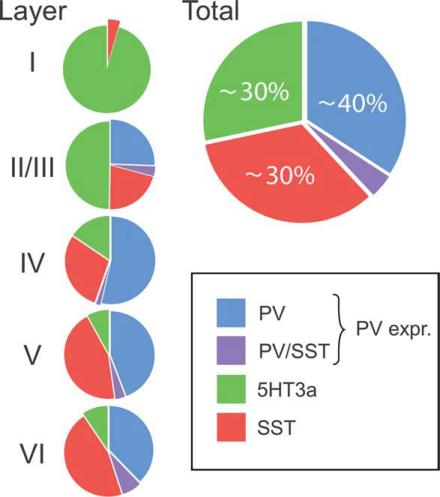
\includegraphics[width=0.4\textwidth]{GABADistribution.pdf}
	\caption{Distribution of GABAergic interneurons in S1
        cortex by immunohistological marker. Reproduced from
        \cite{Rudy2011}.}
	\label{GABADistribution}
\end{figure}


\subsubsection{Connectivity between different cell types}

In order to gain an understanding of the circuits the different
interneuron cell types are involved in, it is important to consider
their interconnectivity. Several studies have sought to determine the
connectivity between Pv-ir, Sst-ir and other interneuron types. The
core findings of these studies determined that Pv-ir cells
preferentially inhibit one another, Sst-expressing cells avoid one
another and inhibit all other types of interneurons particularly the
Pv-ir cells \citep{Xu2013}, while a third type, the Vip-ir cells
preferentially inhibit Sst-ir cells \citep{Pfeffer2013}. This
connectivity profile is schematically represented in Figure
\ref{gaba_circuit}. In mouse cortex the Pv-ir, Sst-ir and Vip-ir cells
accounted for about 40\%, 18\% and 8\% of the GABAergic population,
respectively \citep{Xu2010}, and although these percentages vary
considerably across species Pv-ir and Sst-ir are always the two most
commonly expressed GABAergic populations.

\begin{figure}
	\centering
        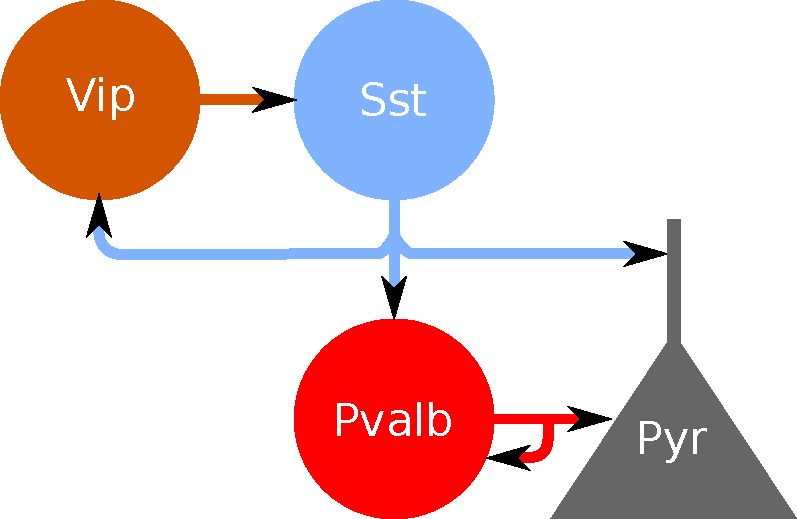
\includegraphics[width=0.7\textwidth]{pfeffer_gabacircuit.pdf}
	\caption{Connectivity between somatostatin (Sst),
        parvalbumin (Pv), vasoactive intestinal peptide (Vip)
        expressing and pyramidal (Pyr) cell types. Adapted from
        \cite{Pfeffer2013}.}
	\label{gaba_circuit}
\end{figure}

Recent tracing techniques have also been able to establish that
excitatory cells provide orientation specific inputs to the inhibitory
population. Using viral tracing techniques \cite{Liu2013} are able to
trace inputs to inhibitory and excitatory neurons in the cat visual
cortex.

\section{Interactions between neuromodulators and V1 circuitry}

As the prime interest of this report and the PhD project is to
characterize the influence of cholinergic modulation on V1 circuitry,
this section will detail how cholinergic basal forebrain inputs may be
modulating the different cell types described above and how this may
give rise to the effects that were described in the PhD proposal. It
will also try to provide a general framework of cholinergic
modulation.

As outlined in the previous report there are two main groups of
acetylcholine receptors (AChRs), nicotinic and muscarinic, hereto
referred to as nAChRs and mAChRs, respectively. While nAChRs are
primarily expressed presynaptically on thalamocortical afferents,
mAChRs are expressed throughout the cortex on a large variety of cell
types with highly divergent effects. The recent review by
\cite{Thiele2013} provides a thorough summary on the effects of
muscarinic and cholinergic signaling within neocortical circuits,
highlighting the fact that the data is still relatively sparse, often
contradictory and do not yet point to a definite theory of cholinergic
modulation. However, in addition to laying out the evidence,
summarized in the schematics shown in Figure \ref{ach_circuit}, two
main theories of cholinergic modulation of neocortical circuits are
discussed. The influential theory that cholinergic signaling simply
reduces intracortical processing in favor of feedforward processing is
assessed as simplistic, although it may provide a good first
approximation of the effects. As an alternative, Thiele suggests that
it may be involved in enabling efficient filtering of information to
satisfy current task demands but points out this theory too needs
further refinement. By identifying the core circuits affected by
cholinergic signaling it may be possible to close in on a more refined
framework and refine current theories.

\begin{figure}
	\centering
        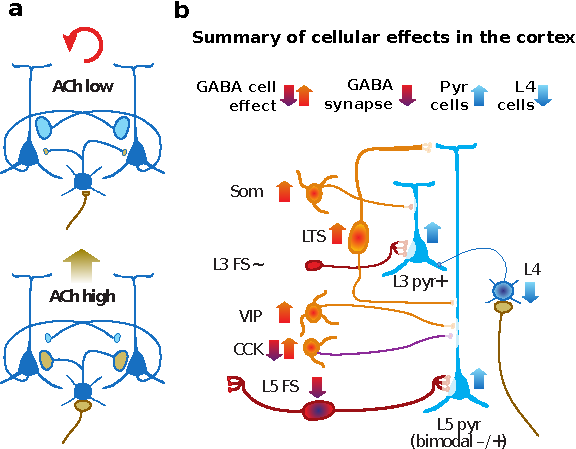
\includegraphics[width=0.7\textwidth]{ach_circuit_effect.pdf}
	\caption{Cholinergic effects on cortical circuits. (a)
        Cholinergic effects on the processing of feedforward versus
        internal information. When acetylcholine (ACh) is low,
        synaptic efficacy of intrinsic connections is high, while
        feedforward synaptic efficacy is average. Therefore,
        information flow is dominated by recurrent processing. When
        ACh is high, feedforward synaptic efficacy is high (through
        presynaptic nicotinic mechanisms), while synaptic efficacy of
        intrinsic connections is reduced (through M2-type receptor
        mediated mechanisms). In this mode, processing is dominated by
        feedforward information. (b) Overview of muscarinic effects on
        cortical circuitry, which may enable efficient filtering of
        information. Arrows indicate whether neuronal activity is
        increased or decreased by muscarinic signaling. Reduced
        intensity of colors at synaptic sites indicates that the
        synaptic efficacy is reduced by muscarinic signaling. The
        diagram does not provide immediate insight into the likely
        consequences of the effects, but rather intends to give a
        graphic overview of the main effects reported in the
        literature. Reprinted from \cite{Thiele2013}.}
	\label{ach_circuit}
\end{figure}

In order to begin modeling the effects of cholinergic modulation and
possibly shed some light on the different frameworks of their action,
it is important to establish their effect on the different cell
classes that have been identified and characterized hereto. In the
mammalian neocortex both mAChRs, in their m1 and m2 subtypes
\citep{Tigges1997}, and nAChRs \citep{Han2000} are expressed at
significant levels. Nicotinic AChRs are primarily expressed
presynaptically in thalamic axons arriving in primary sensory areas
and have been shown to boost the response gain of layer 4C principal
neurons \citep{Disney2007,Gil1997}. In layers 2,3 and 5 on the other
hand, the main effect of nicotinic application seems to be general
suppression mediated by nAChR expression on different interneuron
classes.

Muscarinic AChRs are strongly expressed in different GABAergic
populations but particularly among Pv-ir neurons, which show strong
expression of the m1 receptor subtype in their somata (87\% of cells)
and much weaker expression of the M2-subtype 31\% of cells), which was
generally restricted to the axons \citep{Disney2008}. Surprisingly
however several studies have indicated that the intrinsic excitability
of FS cells is unaffected by cholinergic agonists
\citep{Gulledge2007,Kruglikov2008}. Conversely synapses by FS cells
onto pyramidal cells in layers 3, 4 and 5 seem to be strongly
downregulated through an M2-receptor mediated mechanism
\citep{Kruglikov2008}, which may powerfully reduce feedforward
inhibition. At the same time it remains unclear what role the strong
somatic expression of m1-AChRs may serve in modulating Pv-ir
responses. Non-FS interneuron to pyramidal cell connections also seem
to be downregulated by cholinergic modulation \citep{Yamamoto2010},
while there seems to be a strength dependent effect on
inter-interneuronal connections, whereby weak connections are
strengthened while strong connections are weakened, indicating that
cholinergic modulation of GABAergic synaptic transmission is
differentially regulated depending on the postsynaptic neuron subtype
and connection strength. To underscore these diverse effects,
muscarinic-induced activation of both Sst-ir and ViP-ir cells has been
observed \citep{Kawaguchi1997}.

In the spiny neuron population there also seems to be significant
heterogeneity among modulatory effects. In rat barrel cortex for
example, m4-AChR receptor activation causes hyperpolarization among
layer 4 spiny neurons, which effectively reduces onward communication
\citep{Eggermann2009}. On the other hand, through m1-receptor mediated
effects layer 2/3 and layer 5 pyramidal cells are depolarized
\citep{Eggermann2009}, which would result in filtering out of weak
signals impinging on thalamocortical recipient neurons, while onward
communication is boosted. Recurrent excitation on the other hand seems
to be reduced through both nicotinic and muscarinic pathways
\citep{Levy2006}. Interestingly the nicotinic pathway seems to reduce
recurrent excitation in an activity dependent manner, due to its
dependence on NMDA receptor activation.

As can be seen the effects of nAChR and mAChR activation on cortical
circuits is highly complex and far from fully characterized. However
several clear effects of acetylcholine on V1 circuitry can be
identified:

\begin{itemize}
  \item Thalamocortical synapses onto layer 4 spiny neurons are
    boosted in efficacy.
  \item Layer 4 spiny stellate cells are suppressed filtering out weak
    inputs.
  \item Layer 2/3 pyramidal cells are facilitated, amplifying signals
    arriving from layer 4.
  \item FS basket cell responses are mostly unaffected but their
    synaptic GABA release is suppressed through axonal m2-receptor
    activation.
  \item Sst-ir cells are depolarized through muscarinic receptor
    activation.
  \item Recurrent excitation is reduced through both muscarinic and
    nicotinic mechanisms.
\end{itemize}

\section{GABAergic regulation of plasticity and column structure}

Experience dependent plasticity has been shown to shape the
organization of the sensory cortex during the critical period and
beyond. Dark rearing \citep{Fregnac1978} and monocular deprivation
(MD) experiments \citep{Shatz1978} in particular have confirmed the
fundamental importance of sensory experience in shaping the
development of the cortex. The mechanisms controlling the onset of the
critical period and regulation of plasticity thereafter have also been
studied extensively and a large body of evidence points to the
important role of the inhibitory neurotransmitter
$\gamma$-aminobutyric acid (GABA) in regulating synaptic
plasticity. However as the above paragraphs have shown the population
of GABAergic neurons is highly heterogeneous with hugely divergent
anatomical and functional profiles. Using specific pharmacological and
genetic populations it has been possible to narrow down the
involvement of certain interneuron subtypes in shaping critical period
plasticity and column structure in the cortex.

One of the first indications that GABAergic circuits are involved in
shaping plasticity came when it was shown that a gene-targeted
disruption of the GABA synthetic enzyme glutamic acid decarboxylase 65
(GAD65) could delay critical period onset indefinitely
\citep{Fagiolini2000}. In order to further narrow down the specific
GABA circuits underlying visual cortical plasticity, more specific
pharmacological manipulations were required. On that basis
\cite{Fagiolini2004} used benzodiazepine infusions, known to
selectively enhance GABA type A ($GABA_A$) receptor-mediated currents
through the $\alpha1$ subunit \citep{Rudolph1999}, in conjunction with
MD to prematurely trigger ocular dominance plasticity in mice. These
$GABA_A$ receptor-$\alpha1$ subunits are preferentially enriched at
somatic synapses receiving input from Pv-ir large basket cell
terminals \citep{Klausberger2002}, strongly implicating large basket
cells in visual cortical plasticity.

Beyond controlling the timing of critical period plasticity further
experiments using benzodiazepines have shown strong effects on the
columnar organization of the cortex. The experiment by
\cite{Hensch2004} locally infused regions of cat area 17 with the
$GABA_A$ agonist diazepam and an inverse agonist (DMCM) and studied
the effects on the ocular dominance columns. Chronic treatment with
diazepam had little effect in the functional properties of mature
cortical neurons in vivo apart from enhancing inhibitory postsynaptic
currents. However, the treated hemisphere exhibited reduced
binocularity of single unit responses and wider OD columns near the
infusion site. Infusion with the benzodiazepine inverse agonist DMCM
had the inverse effect, resulting in less discrete and narrower
columns near the infusion site. These results suggest that the
diazepam mediated enhancement in competition reduces binocularity of
single-unit responses, as well as sharpening and widening the
anatomical segregation of monocular regions near the infusion
site. This once again suggests that $GABA_A$ inhibitory currents,
primarily originating from Pv-ir neurons in the cortex, are
fundamentally important to shaping the plasticity and organization of
the cortex.

In order to establish how ocular dominance plasticity emerges during
monocular deprivation, \cite{Kuhlman2013} developed even more
precisely targeted pharmacological manipulations. By selectively
expressing specific receptors on Pv-ir cells they were able to
selectively up- and down-regulate their activity. Their results
indicate that a rapid, but transient reduction in Pv-ir cell firing
restores pyramidal cell firing to pre-deprivation levels allowing
competitive plasticity to occur. Pv-ir neurons therefore seem to play
a permissive role in visual cortical plasticity. Interestingly adult
sensory plasticity such as reinforced associative learning occurs
through a similar mechanism, where cholinergic activation of layer 1
interneurons suppresses Pv-ir neural activity allowing associative
fear learning to occur \citep{Letzkus2011}. All this work suggests a
crucial role for Pv-ir neurons in controlling cortical plasticity
during the critical period and beyond.

\section{Functional Roles of Intracortical Connectivity}

A major feature of the neural code in the cortex is the elimination of
redundancy in order to achieve a sparse representation of the input or
if there is insufficient information to fill in the missing
information based on remembered statistics of the visual world. Sparse
coding in developmental models of the primary visual cortex can be
achieved by allowing lateral inhibitory connections to develop
non-isotropic connectivity, which allows the network to learn the
redundant features of the input and suppress them. If such development
is not allowed to take place and isotropic surround suppression is
employed, cross-orientation stimuli, belonging to a separate object or
contour may be suppressed, thus reducing the information content
encoded by the network. Therefore long-range isotropic suppression has
to be considered destructive \citep{Miikkulainen2005b}. Similarly,
strong lateral excitation will activate neural ensembles representing
non-existing inputs based solely on previous input statistics. While
this is desirable when very little information is available it can
disrupt sparse code formation by expanding the activity bubble or
causing the false detection of a stimulus. Therefore the sensory
cortex has to maintain a fine balance not only between excitation and
inhibition but also in combining past information with the feedforward
information stream arriving in the cortex. Identifying and modeling
the circuits involved in these processes is a fundamental challenge
for neuroscience and will hugely contribute to extending our
understanding of cortical information processing.

Over the last decade evidence for multiple separate inhibitory
populations, subserving different functions, has been considerably
strengthened. Although their precise properties in regard to
morphological and electrophysiological heterogeneity are still unclear
there are a number of identifiable circuit elements. Afferent input
provides strong, low latency excitation to the Pv-ir neurons in the
thalamocortical recipient layer 4, which in turn act as both a
feedforward inhibition and dynamic gain control mechanism on the
broadly activated excitatory cell population. This results in local
decorrelation of the neural activity, which allows recurrent
excitation to amplify the activity in the local neural
ensemble. Meanwhile Sst-ir neurons begin to integrate the local
activity through the local and long-range orientation-specific lateral
connections. If their inputs are sufficiently strong they will
activate allowing this polysynaptic circuit to reduce long range
correlation in the input activity, further reducing redundancy. If
they are only weakly activated on the other hand, long-range lateral
excitatory connections aren't outcompeted and the circuit can fill in
weak or missing information based on past statistics. Under such
regimen the differential recruitment of the two separate inhibitory
populations would be responsible for a shift in cortical state from a
mode of redundancy-reduction and feature discrimination to one of
visual inference. Additionally, modulatory inputs to the cortex like
cholinergic modulation arriving from the nucleus basalis may mediate a
number of effects, whether that is a shift in the circuit from a
down-state, where information is recurrently processed, to a
feedforward heavy up-state, by reducing feedforward inhibition and
boosting feedforward excitation, or a mode in which task-relevant
information is selectively filtered, is still unclear. The following
sections will outline how these possibilities have begun to be
explored by constructing a model based on the available experimental
evidence and will outline plans to begin testing some of these
different hypothesis.

\section{Contextual Modulation and Attention}

The computational task in vision is to map visual experience to the
cortical representation of that particular stimulus or if no such
representation exists, to extract lower level features in order to
encode them for future reference. Using this statistical model the
brain is then able to decide, which visual features carry behavioral
importance and which can be safely ignored. As such the neocortex has
to combine prior information with the incoming information stream and
quickly and reliably identify the most salient stimuli. It has often
been argued that this process is mediated by bottom-up and top-down
processes, although it seems likely that there is close coupling
between the two. This section will outline high level models of
attentional modulation, attempts to understand the neurobiological
processes behind them and more basic contextual modulation phenomena
may underly many of these higher level effects.

\subsection{Models of Attentional Modulation}

The advent of the predictive coding theory of cortical information
processing formalized by Rao and Ballard \citep{Rao1999} suggests that
incoming visual information is combined with encoded natural image
statistics inherent in the feedforward and lateral connections of the
cortex in a process similar to Bayesian inference. Since then a number
of papers have linked attention to surprise and uncertainty
\citep{Feldman2010,Itti2009,Rao2005,Yu2005}, suggesting that it acts
as a mechanism to reduce uncertainty by combining stimulus related
activity and internal priors in a probabilistic manner. A theory of
attentional modulation that can account not only for specific
attention related effects but also resolve some of the
implementational details of predictive coding and the various routing
problems associated with the hierarchical organization of the cortex
would be of tremendous interest.

The number of algorithmic models of attention range from relatively
unspecific descriptive models, such as the attentional spotlight
analogy \citep{Posner1980}, to functional models such as the
relatively recent normalization based structural models by
\cite{Reynolds2009} and \cite{Lee2009}. The list of models of
attention is seemingly endless so it is infeasible to provide even a
grazing overview, but after a long history of descriptive models
perhaps one of the most widely recognized models of attention has been
the so called biased competition model by \cite{Desimone1995}, in
which they suggest that objects in the visual field compete for
control of behavior through both top-down and bottom-up
mechanisms. While top-down mechanisms select objects of behavioral
relevance, bottom up mechanisms separate salient stimuli from their
background.

Another widely recognized model of attention is feature similarity
gain \citep{Treue2001} later extended to feature based attention
\citep{Maunsell2006}, which suggests that attention adjusts the gain
of each neuron depending on the similarity between the observed
stimulus and currently attended feature. The more recent normalization
model of attention proposed by \cite{Reynolds2009} combines the
predicted effects of both into one relative simple mechanism, which is
to multiply the stimulus related activity by an attentional field, the
result of which is then normalized by the aggregate suppressive
drive. In particular, it predicts a dissociable effect of contrast and
attentional modulation, which has since been confirmed by various
studies \citep{Lee2009, Pooresmaeili2010}. Further, the suggestion
that normalization can be applied not only spatially but also in other
stimulus feature dimensions raises the possibility that spatial
attention is just a subset of feature attention.

These types of mechanisms also have some links to the predictive
coding theory of cortical computation as they provide a mechanism of
combining stimulus related activity with prior information encoded in
the lateral and feedback connections. A paper by \cite{Spratling2010}
formalizes this mechanism as a true predictive coding model by
modeling the primary visual cortex through an interaction between
afferent inputs, which compete with predictive neurons acting through
divisive feedback to represent the stimulus in error-coding
neurons. Although these models are successively more predictive none
truly begins to explains what neural mechanisms underly these
processes. Although a complete description at this level will be
beyond reach for some time it may be possible to start linking these
processes back to their neurobiological implementation in the brain.

\subsection{Theory of Cholinergic Modulation and Attention}

Although there are very few models addressing attention at the
implementational level, much more is known about the neurobiology of
attention than just a few years ago. Information from the RF center
and the surround is integrated in a process heavily mediated by
neuromodulators and feedback connections including those involved in
attention.

Contextual influences mediated through lateral connectivity have been
closely associated bottom-up attention possibly representing learned
priors of natural image statistics established through development and
learning \citep{Series2004}. In addition, a number of studies have
implicated cholinergic, noradrenergic and glutamatergic
neurotransmitter pathways in modulating FF thalamo-cortical, lateral
intra-areal and FB intracortical connections.

In a recent review paper, \cite{Harris2011} argue that the brain and
the neocortex in particular constantly adapts how information is
integrated and routed. Although they focus primarily on cortical
states, synchrony and other temporal phenomena, the review identifies
a number of structures involved in modulating processing in the cortex
(visualized in Figure \ref{FBThiele}). This includes cholinergic
projections from the cholinergic nuclei in the brain stem and the
basal forebrain, noradrenergic projections from the locus coerulus and
serotonergic projections from the Raphe nucleus targeting cortical and
subcortical visual areas. In addition to these extracortical feedback
connections, Harris and Thiele argue that glutamatergic feedback
connections from the frontal eye fields (FEF) project down along the
cortical visual hierarchy inducing shifts in attention at the
behavioral and neuronal level. Overall this line of argument suggests
that the interaction between all these feedback projections with their
cortical targets provide the substrate for shifts in cortical state
and attention.

\begin{figure}
	\centering 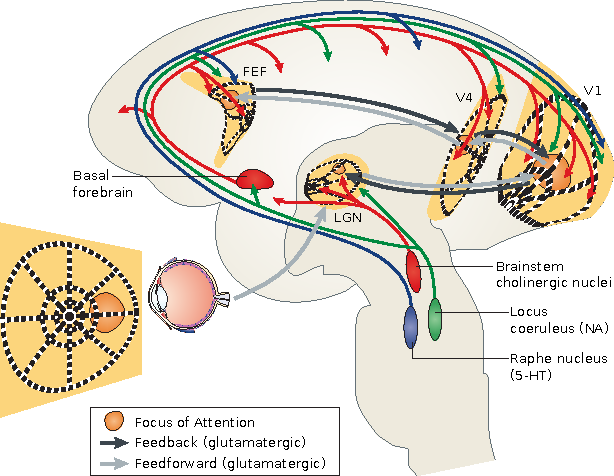
\includegraphics[width=1.0\textwidth]{FBThiele.pdf}
	\caption{Proposed mechanisms for desynchronisation during
        state changes and attention. Taken from \cite{Harris2011}.}
	\label{FBThiele}
\end{figure}

In order to provide a coherent theory of what these neuromodulators
are doing it is once again paramount to bind experimental observations
together in a framework that is concerned with the computational
purpose of the system. Before attempting to understand the precise
physiology and action of individual neurotransmitter pathways, which
are far from fully being fully understood, let's consider their action
in the larger computational framework of predictive coding. Although
still rather tentative, \cite{Yu2005} argue that acetylcholine and
noradrenaline act as signaling mechanisms for the coding of
uncertainty, forming a crucial part in the cortical inference
algorithm hypothesized by the predictive coding theory. They
hypothesize based on a number of observations that acetylcholine
signals, what they describe as expected uncertainty, while
noradrenaline signals unexpected uncertainty. While the distinction
isn't always clear cut, broadly speaking expected uncertainty refers
to situation where a certain cue isn't entirely reliable and therefore
needs to be scrutized in high detail without necessarily relying on
the inherent predictions of the cortex, while unexpected uncertainty
would arise when the predictive capacity of a variable is suddenly
severely compromised necessitating a shift or refocusing of attention.

\subsection{Mechanisms of Visual Attention}

Acetylcholine has been implicated in a number of cognitive functions
including excitability, attention, learning, memory, wake and sleep
cycles and cortical modulation of sensory information processing. It
is unclear how the cholinergic system regulates or at the very minimum
modulates this wide range of functions, so it is important to get a
thorough understanding of its different mechanisms of action at the
channel, synaptic, cellular and network level.

The cholinergic pathways (Ch1-Ch6) originate in the the basal
forebrain, which itself has been implicated in global attention and
arousal states \citep{Jones2004}. The nucleus basalis provides
cholinergic input to a number of brain areas including the cortex and
the thalamus, which has been through the Ch5-6 and Ch4 pathways
respectively. The cortical pathway (Ch4) mainly originates from the
nucleus basalis magnocellular (NBM) with a topographic organization
\citep{Woolf1991}. In addition, labeling studies have identified small
populations of cholinergic bipolar intracortical interneurons in layer
2/3 of the cortex \citep{vonEngelhardt2007}. Among population of
neurons in the NBM projecting to the cortex 30-25\% are GABAergic
neurons, whose axons primarily target cortical GABAergic interneurons
acting to disinhibit them \citep{Lucas-Meunier2003}. The remainder
release ACh in the cortex, a process which is regulated by modulation
of cholinergic neurons in the NBM or by cholinergic terminals in the
cortex.

Acetylcholine receptors in the cortex can be roughly classified into
nicotinic and muscarinic AChRs. The nicotinic and muscarinic AChRs are
differentially expressed in neuronal subtypes with mAChRs being more
commonly found in inhibitory intracortical neurons \citep{Disney2006},
while nAChRs have been determined to be preferentially expressed
pre-synaptically in the thalamo-cortical recipient layer 4C of V1
\citep{Disney2007}. Nicotinic receptors are permeable to $Na^+$, $K^+$
and $Ca^{2+}$ ions, with particular permeability to $Ca^{2+}$, which
can cause rapid increases in intracellular $Ca^{2+}$ concentration and
thus influence cellular $Ca^{2+}$-sensitive processes
downstream. Through this mechanism and their presynaptic positioning,
nAChRs can modulate neurotransmitter release
\citep{Lucas-Meunier2003}, which has been found to effect a
multiplicative response gain enhancement in layer 4C
\citep{Disney2007}. The muscarinic receptor type itself has several
genetically defined subtypes, namely m1-m5. Of these the m1 and m2
AChRs are known to be strongly expressed in primates and correspond to
the two pharmalogically classes of mAChRs, M1 and M2
\citep{Disney2006}. In the neocortex mAChRs exhibit a clear laminar
distribution with strong expression primarily in layers 2/3 and 5. It
was found that GABAergic neurons primarily expressed the m1 subtype,
where they are usually found expressed somatically, while
glutamatergic neurons primarily express mAChRs dendritically
\citep{Lucas-Meunier2003}. Further it seems as if mAChR expression on
glutamatergic neurons is relatively low in lower visual areas,
increasing in V2 relative to V1, suggesting ACh primarily acts through
inhibitory mechanisms in V1. This has been affirmed by a recent study
showing that ACh suppresses response gain outside of layer 4C, by
strengthening inhibition \citep{Disney2012}. In the past it was
thought this suppressive effect is mediated by m2-type mAChRs, which
act to reduce glutamate release
\citep{Hasselmo2004,Roberts2005,Yu2005} but the expression data seems
to contradict this. More recent studies indicate that the ACh mediated
suppression is caused almost entirely by increased GABA release and
GABA$_A$ receptor activation, itself driven by m1-type mAChR
activation. This hypothesis would also account for the observation
that attentional effects are weakest in area V1, where mAChR
expression on glutamatergic neurons is weakest, increasing in strength
as one moves up the cortical hierarchy \citep{Disney2006}. Nonetheless
\cite{Soma2012} found substantial mAChR-mediated response gain
enhancement even in area V1, suggesting ACh much like attention can
mediate significant facilatory and suppressive effects in V1.

At the subcortical level, experiments by \cite{Goard2009} showed that
response reliability was improved through a pathway acting on the LGN
projecting from the basal forebrain indirectly either through
cortico-thalamic or a pathway involving the reticular thalamic nucleus
(RTN), which has been called ``gatekeeper'' of the LGN. The feedback
loop involving the nucleus basalis, RTN and LGN seems most likely to
be involved in very coarse gating of the visual stream such that a
modelling approach could assume a fully aware state in which thalamic
gating is ignored. This reduces the initial scope of this project to
the action of a particular neurotransmitter in a particular region of
the brain, namely acetylcholine and the primary visual cortex,
although it may well be extended at a later stage.

\begin{figure}
	\centering
        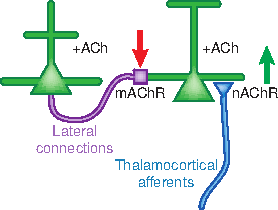
\includegraphics[width=0.5\textwidth]{achreceptors.pdf}
	\caption{Diagram showing the synaptic locus of nicotinic
        and muscarinic ACh receptors in cortical circuits
        \citep{Thiele2009a}.}
	\label{AChRs}
\end{figure}

A number of studies have noted and investigated the similarity in the
activation profiles of cholinergic innervation and attentional
modulation in V1.  This seems to be backed up by evidence that shows
that much like attention, topical acetylcholine application reduces
the effect of long-range lateral connectivity, thereby reducing
spatial summation \citep{Roberts2005}, suppressing contextual
influences and effectively decorrelating the cortical activity
\citep{Goard2009}. Further investigation concluded that these
attention-mediated changes in spatial integration are
eccentricity-dependent such that spatial summation is reduced in the
parafoveal regions and expanded in more peripheral visual areas
\citep{Roberts2007}. Additionally it was shown that ACh causes a
broadening of orientation tuning in a majority of cells, while only
sharpening them in a small number of other cells
\citep{Zinke2006}. Research by \cite{Soma2012} has delineated the
effects of muscarinic and nicotinic AChR activation on response gain,
showing mAChR activation in particular mediates a significant increase
in response gain, which could be almost completely blocked by applying
an mAChR antagonist and any residual effects could be removed by
blocking both m- and nAChRs. A limited effect of nAChR activation on
increases in the mean firing rates was also demonstrated by further
studies \citep{Herrero2011}, although mAChR blockade was shown to have
the opposite effect. The same study found that mAChR activation was
distributed equally among layers except layer 4C, in which nAChR
activity dominates. Finally a substantial amount of evidence has
accumulated showing that ACh also reduces the Fano factor, i.e. the
firing rate variability \citep{Herrero2011}. This provides clear
evidence of ACh on orientation tuning, spatial summation, response
gain modulation and firing rate variability, effects closely
associated with attention.

The precise influence of acetylcholine on surround modulation has at
times been hard to discern as there are a number of effects to be
delineated. Broadly speaking surround modulation can be broken down
into facilatory and inhibitory effects acting over different spatial
and time scales and differentially activated by different contrasts,
eccentricities and stimulus features. As stated before both attention
and iontophoretic ACh application were shown to reduce spatial
integration \citep{Roberts2005,Roberts2007} and mAChRs were found to
be expressed largely on intracortical neurons thought to be involved
in spatial summation beyond the cRF. Additionally some evidence seems
to indicate ACh alters the membrane spatial and temporal integration
constants \citep{Lucas-Meunier2003} further complicating the
dissociation of mechanisms. A number of studies have nonetheless
attempted to classify the effects on both colinear facilitation and
suppression. In particular, counter to initial theoretical
considerations, it seems flanker induced surround suppression is
actually facilitated by mAChR activation, as their blockade was shown
to reduce the suppressive drive \citep{Herrero2011}. The effect on
surround facilitation was similar although several studies noted that
only very few neurons exhibited flanker induced facilitation in the
first place \citep{Pooresmaeili2010}. So although in theory almost
everyone agrees that both attention and acetylcholine boost
feedforward information and reduce spatial integration and
extra-classical surround effects, it is unclear under which conditions
these effects can be observed and what mechanisms drive them.

A particular issue that has not yet been resolved is the discrepancy
between the highly localized effect of attentional neuromodulation and
the comparatively coarse effect of ACh innervation. Suggested
resolutions to this problem include the recent discovery of
cholinergic interneurons \citep{vonEngelhardt2007}, found in layer 2/3
of V1 as well as interactions with spatially specific glutamatergic
feedback connections \citep{Herrero2008,Sarter2009}. Overall however
it seems evidence is strong that both nAChRs and mAChRs are involved
in mediating activity in V1 by boosting feedforward activity from the
thalamus and modulating the spatial integration of V1 neurons with
efferent connections to higher layers with clear data as to the
contribution of each.

Overall the entire mechanism of attentional feedback is poorly
understood and it makes sense to focus particularly on the aspects
that can easily be implemented in a powerful yet simple
model. Cholinergic signalling in V1 provides exactly such a target
system as it has been implicated in a number attention mediated
effects and can be straightforwardly translated into their mechanisms
of action, one reducing the effect of long range contextual influences
on V1 receptive fields, thereby decorrelating the input and secondly a
gain mechanism boosting behaviourally relevant signals in the
thalamo-cortical connections. Additionally, it seems to interact with
glutamatergic feedback connections from higher cortical areas, further
expanding the range of interactions that can be investigated.

\subsection{Contextual and Attentional Phenomena in V1}

A number of phenomena associated with attention and contextual
modulation, including iso-orientation suppression or facilitation,
boundary detection, contour completion and noise exclusion have been
observed in V1. Although these phenomena are generally associated with
bottom-up attention they lay the foundation for higher level phenomena
such as pop-out and figure-ground segregation and may reveal more
about general mechanisms applying also to higher visual areas.

Basic contextual effects such as iso-orientation suppression have
already been discussed and models have begun to suggest the functional
connectivity mediating implicating both lateral and feedback
connections. While, \cite{Li2002} has proposed that pre-attentive
bottom-up processes allow V1 to generate a saliency map of the visual
input. However, the fact that higher cortical areas have also been
associated with saliency signaling and the lack of long range
intra-areal connectivity in V1 suggest that while it can encode local
saliency, feedback is required to globally integrate saliency across
visual space.

Feedback modulation of V1 activity has been implicated in a number of
effects, spatial attention being chief among them. Spatial attention
is thought to be able to select multiple low and high level objects in
the visual space across V1 and higher visual areas
\citep{McMains2004}. It is thought to underly noise exclusion,
observed by \cite{Dosher2000} and may be explained by effects similar
what has been experimentally observed during ionphoretic application
of ACh. Other effects that have been commonly been associated with
feedback in some form are the signaling of illusory contours, which
have been shown to be negatively signaled or deemphasized in V1
\citep{Ramsden2001} and boundary detection \citep{Poort2012}.  In the
planning section, concrete proposals will be made suggesting what
mechanisms may account for these phenomena and how they can be
implemented.

\section{Natural Image Statistics, Sparsity and Horizontal Connections}

It has long been hypothesized that connectivity in the cortex captures
the statistics of the sensory input in order to perform predictions
and maintain sparse representations of novel inputs
\citep{Simoncelli2001}. A wide range of work has explored the role of
the distributions of light intensities, color statistics and spatial
correlations in natural images. In particular, the power law
distribution of spatial frequencies in natural images has been widely
discussed in the literature but ultimately this largely seems to
reflect the scale invariance within natural images
\citep{Ruderman1997}.

Numerous studies and models have since been devised to address whether
the visual system takes advantage of the correlational structure of
natural images. These types of normative models were able to show that
surround inhibition, whether subtractive or divisive, could cancel out
correlations effectively whitening or decorrelating the activity in
the visual system \citep{Srinivasan1982, Atick1992}. In doing so they
quickly found that simple decorrelation wasn't sufficient to optimally
represent natural images because whitening does not eliminate all
structure in a natural image, e.g. edges and lines remain. By
introducing an explicit sparsity constraint, \cite{Olshausen1996} were
able to develop V1-like simple cell receptive fields with varying
orientations, spatial frequencies and sizes. These models indicated
that sensory system was optimizing two contstraints, sparsity and
statistical independence. However, even these approaches cannot
achieve complete statistical independence since there are higher order
correlations even between non-overlapping receptive fields.

By introducing divisive normalization, \cite{Schwartz2001a} were able
to show that these types of dependencies could be further
eliminated. Furthermore, the weights used in the computation of the
normalization signal could be specifically optimized to maximize the
independence of the normalized responses. Additionally, they
demonstrated that the optimal weights were at least partly due to the
prevalence of extended contours in natural images. Attempting to
quantify the co-occurence statistics of contours in natural images,
\cite{Geisler2001} demonstrated that the performance in contour
detection tasks could be predicted by a local grouping rule derived
from the co-occurence statistics. The first explicit link to
horizontal connectivity was made by \cite{Sigman2001}, who noted that
the pattern of long-range patchy connectivity in the primary visual
cortex, linking iso-orientation columns has a close corespondence with
the observation of co-circularity in natural image statistics. Noting
the processes of iso-orientation suppression and contour integration,
they argue that iso-orientation suppression may serve to further
reduce redundancies in neural coding, thereby achieving greater
statistical independence, which would explain why neural responses
appear most sparse when presented with natural stimuli. Secondly,
observing that visual cortex can also exhibit colinear faciliation
under low contrast conditions \citep{Sceniak1999, Kapadia1999}, they
suggest that under low signal-to-noise conditions the cortex may act
to enhance repeated statistics to aid the identification of contours
and form.

These theoretical studies have hugely advanced our thinking about the
computations performed by the early visual cortex, however very little
work has been done to look at the actual structure of horizontal
connectivity in V1, largely due to the difficulty in obtaining data
from more than just a few cells. Even on the question whether
horizontal connections are anisotropic along the axis of preferred
orientation of the neuron, as would be expected from theoretical
studies, there is conflicting evidence. The result has been confirmed
in monkey \citep{Sincich2001}, tree shrew \citep{Bosking1997} and cat
\citep{Schmidt1997}, but conflicting results exist in macaque
\cite{Angelucci2002}. By performing analyses on an old tree shrew
dataset \cite{Hunt2011} investigated whether horizontal connections
captured the co-circularity of natural image statistics. Although they
found neurons, which exhibited co-circularity and anti-cocircularity
and hypothesize a role for both, given the small number of lateral
connections fields and the fact that second order properties are
highly sensitive to even small errors in the data, it is unclear how
strong this result is. Further research in this area is desperately
needed.
